%%%%%%%%%%%%%%%%%%%%%%%%%%%%%%%%%%%%
% Slide options
%%%%%%%%%%%%%%%%%%%%%%%%%%%%%%%%%%%%

% Option 1: Slides with solutions

\documentclass[slidestop,compress,mathserif]{beamer}
\newcommand{\soln}[1]{\textit{#1}}
\newcommand{\solnGr}[1]{#1}

% Option 2: Handouts without solutions

%\documentclass[11pt,containsverbatim,handout]{beamer}
%\usepackage{pgfpages}
%\pgfpagesuselayout{4 on 1}[letterpaper,landscape,border shrink=5mm]
%\newcommand{\soln}[1]{ }
%\newcommand{\solnGr}{ }

%%%%%%%%%%%%%%%%%%%%%%%%%%%%%%%%%%%%
% Style
%%%%%%%%%%%%%%%%%%%%%%%%%%%%%%%%%%%%

\usetheme{metropolis}
%\usetheme{default}

%%%%%%%%%%%%%%%%
% Packages
%%%%%%%%%%%%%%%%

\usepackage{geometry}
\usepackage{graphicx}
\usepackage{amssymb}
%\usepackage{cancel}
\usepackage{epstopdf}
\usepackage{amsmath}  	% this permits text in eqnarray among other benefits
\usepackage{url}		% produces hyperlinks
\usepackage{hyperref}	% allows for color usage in tables
\usepackage[english]{babel}
\usepackage[latin1]{inputenc}
\usepackage{colortbl}	% allows for color usage in tables
\usepackage{multirow}	% allows for rows that span multiple rows in tables
\usepackage{color}		% this package has a variety of color options
\usepackage{pgf}
\usepackage{calc}
\usepackage{ulem}
\usepackage{multicol}
\usepackage{textcomp}
\usepackage{txfonts}
\usepackage{listings}
\usepackage{tikz}
\usepackage{array}
\usepackage{wasysym}
\usepackage{fancyvrb}


%%%%%%%%%%%%%%%%
% Remove navigation symbols
%%%%%%%%%%%%%%%%

\setbeamertemplate{navigation symbols}{}

%%%%%%%%%%%%%%%%
% User defined colors
%%%%%%%%%%%%%%%%

\xdefinecolor{oiB}{rgb}{0.22,0.52,0.72}
\definecolor{oiG}{rgb}{.298,.447,.114}
\xdefinecolor{hlblue}{rgb}{0.051,0.65,1}
\xdefinecolor{gray}{rgb}{0.5, 0.5, 0.5}
\xdefinecolor{darkGray}{rgb}{0.3, 0.3, 0.3}
\xdefinecolor{darkerGray}{rgb}{0.2, 0.2, 0.2}
\xdefinecolor{rubineRed}{rgb}{0.89,0,0.30}
\xdefinecolor{irishGreen}{rgb}{0,0.60,0}	
\definecolor{lightGreen}{rgb}{0.387,0.581,0.148} 

%%%%%%%%%%%%%%%%
% Template colors
%%%%%%%%%%%%%%%%

\setbeamercolor*{palette primary}{fg=white,bg=oiB!80!black!90}
\setbeamercolor*{palette secondary}{fg=black,bg= oiB!80!black}
\setbeamercolor*{palette tertiary}{fg=white,bg= oiB!80!black!80}
\setbeamercolor*{palette quaternary}{fg=white,bg= oiB}
\setbeamercolor{structure}{fg= oiB}
\setbeamercolor{frametitle}{bg= oiB!90}
\setbeamertemplate{blocks}[shadow=false]
\setbeamersize{text margin left=2em,text margin right=2em}

\setbeamercolor{code body}{bg=gray!20!white!80,fg=black}


%%%%%%%%%%%%%%%%
% Get rid of fancy enumerated list bullets
%%%%%%%%%%%%%%%%

\setbeamertemplate{enumerate items}[default]

%%%%%%%%%%%%%%%%
% Custom commands
%%%%%%%%%%%%%%%%

% degree
\newcommand{\degree}{\ensuremath{^\circ}}

% cite
\newcommand{\ct}[1]{
\vfill
{\tiny #1}}

% Note
\newcommand{\Note}[1]{
\rule{2.5cm}{0.25pt} \\ \textit{\footnotesize{\textcolor{rubineRed}{Note:} \textcolor{darkerGray}{#1}}}}

% Remember
\newcommand{\Remember}[1]{\textit{\scriptsize{\textcolor{orange}{Remember:} #1}}}

% expected counts
\newcommand{\ex}[1]{\textit{\textcolor{blue}{#1}}}

% red
\newcommand{\red}[1]{\textit{\textcolor{rubineRed}{#1}}}

% pink
\newcommand{\pink}[1]{\textit{\textcolor{rubineRed!90!white!50}{#1}}}

% green
\newcommand{\green}[1]{\textit{\textcolor{irishGreen}{#1}}}

% orange
\newcommand{\orange}[1]{\textit{\textcolor{orange}{#1}}}

% links: webURL, webLin, appLink
\newcommand{\webURL}[1]{\urlstyle{same}{ \textit{\textcolor{darkGray}{\url{#1}}}}}
\newcommand{\webLink}[2]{\href{#1}{\textcolor{darkGray}{{#2}}}}
\newcommand{\appLink}[2]{\href{#1}{\textcolor{white}{{#2}}}}

% mail
\newcommand{\mail}[1]{\href{mailto:#1}{\textit{\textcolor{darkGray}{#1}}}}

% highlighting: hl, hlGr, mathhl
\newcommand{\hl}[1]{\textit{\textcolor{hlblue}{#1}}}
\newcommand{\hlGr}[1]{\textit{\textcolor{lightGreen}{#1}}}
\newcommand{\mathhl}[1]{\textcolor{hlblue}{\ensuremath{#1}}}

% two col: two columns
\newenvironment{twocol}[4]{
\begin{columns}[c]
\column{#1\textwidth}
#3
\column{#2\textwidth}
#4
\end{columns}
}

% slot (for probability calculations)
\newenvironment{slot}[2]{
\begin{array}{c} 
\underline{#1} \\ 
#2
\end{array}
}

% pr: left and right parentheses
\newcommand{\pr}[1]{
\left( #1 \right)
}

% solnMult: solutions for practice questions

\newcommand{\solnMult}[1]{
\item[] \vspace{-0.59cm}
\only<1>{\item #1}
\soln{\only<2->{\item \orange{#1}}}
}

% cancel
\newcommand{\cancel}[1]{%
    \tikz[baseline=(tocancel.base)]{
        \node[inner sep=0pt,outer sep=0pt] (tocancel) {#1};
        \draw[red, line width=0.5mm] (tocancel.south west) -- (tocancel.north east);
    }%
}

% removepagenumbers
\newcommand{\removepagenumbers}{% 
  \setbeamertemplate{footline}{}
}

%%%%%%%%%%%%%%%%
% Custom boxes
%%%%%%%%%%%%%%%%

% app: application exercise

\setbeamercolor{app body}{fg=oiG}

\newcommand{\app}[1]{
\begin{beamerboxesrounded}[shadow = false, lower = app body]{}
#1
\end{beamerboxesrounded}
}

% dq: discussion question

\setbeamercolor{disc ques body}{fg=oiB}

\newcommand{\dq}[1]{
\begin{beamerboxesrounded}[shadow = false, lower = disc ques body]{}
#1
\end{beamerboxesrounded}
}

% pq: practice question

\setbeamercolor{prac ques body}{fg=oiB}

\newcommand{\pq}[1]{
\begin{beamerboxesrounded}[shadow = false, lower = prac ques body]{}
#1
\end{beamerboxesrounded}
}

% formula

\setbeamercolor{formula body}{fg=oiB!55!black!95}

\newcommand{\formula}[1]{
\begin{beamerboxesrounded}[shadow = false, lower = formula body]{}
#1
\end{beamerboxesrounded}
}


%%%%%%%%%%%%%%%%
% Change margin
%%%%%%%%%%%%%%%%

\newenvironment{changemargin}[2]{%
\begin{list}{}{%
\setlength{\topsep}{0pt}%
\setlength{\leftmargin}{#1}%
\setlength{\rightmargin}{#2}%
\setlength{\listparindent}{\parindent}%
\setlength{\itemindent}{\parindent}%
\setlength{\parsep}{\parskip}%
}%
\item}{\end{list}}

%%%%%%%%%%%%%%%%
% Footnote
%%%%%%%%%%%%%%%%

\long\def\symbolfootnote[#1]#2{\begingroup%
\def\thefootnote{\fnsymbol{footnote}}\footnote[#1]{#2}\endgroup}

%%%%%%%%%%%%%%%%
% Commands from the book
%%%%%%%%%%%%%%%%

\newenvironment{data}[1]{\texttt{#1}}{}
\newenvironment{var}[1]{\texttt{#1}}{}
\newenvironment{resp}[1]{\texttt{#1}}{}

%%%%%%%%%%%%%%%%
% Graphics
%%%%%%%%%%%%%%%%

\DeclareGraphicsRule{.tif}{png}{.png}{`convert #1 `dirname #1`/`basename #1 .tif`.png}



%%%%%%%%%%%%%%%%%%%%%%%%%%%%%%%%%%%%
% Preamble
%%%%%%%%%%%%%%%%%%%%%%%%%%%%%%%%%%%%

\title[Chp 6: Inference for categorical data]{Chapter 6: Inference for categorical data}
\author{OpenIntro Statistics, 3rd Edition}
\institute{$\:$ \\ {\footnotesize Slides developed by Mine \c{C}etinkaya-Rundel of OpenIntro. \\
The slides may be copied, edited, and/or shared via the \webLink{http://creativecommons.org/licenses/by-sa/3.0/us/}{CC BY-SA license.} \\
Some images may be included under fair use guidelines (educational purposes).}}
\date{}


%%%%%%%%%%%%%%%%%%%%%%%%%%%%%%%%%%%%
% Begin document
%%%%%%%%%%%%%%%%%%%%%%%%%%%%%%%%%%%%

\begin{document}


%%%%%%%%%%%%%%%%%%%%%%%%%%%%%%%%%%%%
% Title page
%%%%%%%%%%%%%%%%%%%%%%%%%%%%%%%%%%%%

{
\addtocounter{framenumber}{-1} 
{\removepagenumbers 
\usebackgroundtemplate{
\includegraphics[width=\paperwidth]{../OpenIntro_Grid_4_3-01.jpg}}
\begin{frame}

\hfill 
\includegraphics[width=20mm]{../oiLogo_highres}

\titlepage

\end{frame}
}
}


%%%%%%%%%%%%%%%%%%%%%%%%%%%%%%%%%%%%
% Sections
%%%%%%%%%%%%%%%%%%%%%%%%%%%%%%%%%%%%

%%%%%%%%%%%%%%%%%%%%%%%%%%%%%%%%%%%%

\section{Inference for a single proportion}

%%%%%%%%%%%%%%%%%%%%%%%%%%%%%%%%%%%%

\begin{frame}

\pq{Two scientists want to know if a certain drug is effective against high blood pressure. The first scientist wants to give the drug to 1000 people with high blood pressure and see how many of them experience lower blood pressure levels. The second scientist wants to give the drug to 500 people with high blood pressure, and not give the drug to another 500 people with high blood pressure, and see how many in both groups experience lower blood pressure levels. Which is the better way to test this drug?}

\begin{enumerate}[(a)]
\item All 1000 get the drug
\solnMult{500 get the drug, 500 don't}
\end{enumerate}

\end{frame}

%%%%%%%%%%%%%%%%%%%%%%%%%%%%%%%%%%%%

\begin{frame}
\frametitle{Results from the GSS}

The GSS asks the same question, below is the distribution of responses from the 2010 survey: \\

\begin{center}
\begin{tabular}{l c}
All 1000 get the drug		& 99 \\
500 get the drug 500 don't	& 571 \\
\hline
Total						& 670
\end{tabular}
\end{center}

\end{frame}

%%%%%%%%%%%%%%%%%%%%%%%%%%%%%%%%%%%

\begin{frame}
\frametitle{Parameter and point estimate}

\dq{We would like to estimate the proportion of all Americans who have good intuition about experimental design, i.e. would answer ``500 get the drug 500 don't"? What are the parameter of interest and the point estimate?}

\pause

\begin{itemize}

\item \hl{Parameter of interest:} Proportion of \orange{all} Americans who have good intuition about experimental design.
\[ \mathhl{p}~\scriptsize{(\text{a population proportion})} \]

\pause

\item \hl{Point estimate:} Proportion of \orange{sampled} Americans who have good intuition about experimental design.
\[ \mathhl{\hat{p}}~\scriptsize{(\text{a sample proportion})} \]

\end{itemize}

\end{frame}

%%%%%%%%%%%%%%%%%%%%%%%%%%%%%%%%%%%

\begin{frame}
\frametitle{Inference on a proportion}

\dq{What percent of all Americans have good intuition about experimental design, i.e. would answer ``500 get the drug 500 don't"?}

\pause

\begin{itemize}

\item We can answer this research question using a confidence interval, which we know is always of the form

\[ \textcolor{orange}{point~estimate \pm ME} \]

\pause

\item And we also know that \textcolor{orange}{$ME = critical~value \times standard~error$} of the point estimate.

\[ \mathhl{SE_{\hat{p}} = ?} \]

\end{itemize}

\pause

\formula{Standard error of a sample proportion}
{
\[ SE_{\hat{p}} =  \sqrt{\frac{p~(1-p)}{n}}  \]
}


\end{frame}

%%%%%%%%%%%%%%%%%%%%%%%%%%%%%%%%%%%

\subsection{Identifying when a sample proportion is nearly normal}

%%%%%%%%%%%%%%%%%%%%%%%%%%%%%%%%%%%%

\begin{frame}
\frametitle{Sample proportions are also nearly normally distributed}

\formula{Central limit theorem for proportions}
{
Sample proportions will be nearly normally distributed with mean equal to the population mean, $p$, and standard error equal to $\sqrt{\frac{p~(1-p)}{n}}$.
\[ \hat{p} \sim N \pr{ mean = p, SE = \sqrt{\frac{p~(1-p)}{n}} } \]
}

\begin{itemize}

\item But of course this is true only under certain conditions...

\dq{any guesses?}

\soln{\pause{independent observations, at least 10 successes and 10 failures}}

\pause
\vfill

\Note{If $p$ is unknown (most cases), we use $\hat{p}$ in the calculation of the standard error.}

\end{itemize}

\end{frame}

%%%%%%%%%%%%%%%%%%%%%%%%%%%%%%%%%%%

%\begin{frame}
%\frametitle{A quick activity}
%
%\pq{Flip a coin 20 times -- this is going to get loud! Record the number of heads and then use your clicker to submit the proportion of heads you obtained.}
%
%\begin{enumerate}[(a)]
%\item $\le$ 0.3
%\item 0.4
%\item 0.5
%\item 0.6
%\item $\ge$ 0.7
%\end{enumerate}
%
%\end{frame}
%
%%%%%%%%%%%%%%%%%%%%%%%%%%%%%%%%%%%%

%\begin{frame}
%
%\formula{Central limit theorem for proportions}
%{
%Sample proportions will be nearly normally distributed with mean equal to the population mean, $p$, and standard error equal to $\sqrt{\frac{p~(1-p)}{n}}$.
%\[ \hat{p} \sim N \pr{ mean = p, SE = \sqrt{\frac{p~(1-p)}{n}} } \]
%If the population proportion is not available, use the sample proportion to estimate the standard error.
%}
%
%\pause
%
%Assumptions/conditions:
%\begin{enumerate}[1.]
%\item \hl{Independence}: 
%\begin{itemize}
%\item \hlGr{Random sample}
%\item \hlGr{10\% condition}: If sampling without replacement, $n <$ 10\% of the population.
%\end{itemize}
%\item \hl{Normality}: At least 10 successes and 10 failures.
%\end{enumerate}
%
%\end{frame}
%
%%%%%%%%%%%%%%%%%%%%%%%%%%%%%%%%%%%%

\subsection{Confidence intervals for a proportion}

%%%%%%%%%%%%%%%%%%%%%%%%%%%%%%%%%%%%

\begin{frame}
\frametitle{Back to experimental design...}

\dq{The GSS found that 571 out of 670 (85\%) of Americans answered the question on experimental design correctly. Estimate (using a 95\% confidence interval) the proportion of all Americans who have good intuition about experimental design?}

\pause
Given: $n = 670, \hat{p} = 0.85$. First check conditions.

\pause
\begin{enumerate}[1.]
\item \hl{Independence}: The sample is random, and 670 $<$ 10\% of all Americans, therefore we can assume that one respondent's response is independent of another.
\pause
\item \hl{Success-failure}: 571 people answered correctly (successes) and 99 answered incorrectly (failures), both are greater than 10.
\end{enumerate}

\end{frame}

%%%%%%%%%%%%%%%%%%%%%%%%%%%%%%%%%%%

\begin{frame}

\pq{We are given that  $n = 670, \hat{p} = 0.85$, we also just learned that the standard error of the sample proportion is $SE = \sqrt{\frac{p(1-p)}{n}}$. Which of the below is the correct calculation of the 95\% confidence interval?}

\begin{enumerate}[(a)]
\solnMult{$0.85 \pm 1.96 \times \sqrt{\frac{0.85 \times 0.15}{670}}$} \soln{\only<2>{\orange{$\rightarrow (0.82, 0.88)$}}}
\item $0.85 \pm 1.65 \times \sqrt{\frac{0.85 \times 0.15}{670}}$
\item $0.85 \pm 1.96 \times \frac{0.85 \times 0.15}{\sqrt{670}}$
\item $571 \pm 1.96 \times \sqrt{\frac{571 \times 99}{670}}$
\end{enumerate}

\end{frame}

%%%%%%%%%%%%%%%%%%%%%%%%%%%%%%%%%%

%\begin{frame}
%\frametitle{Interpretation of the CI}
%
%\pq{Based on this confidence interval, does it appear that more than a 80\% of Americans have a good intuition on experimental design? \\
%\soln{(0.82, 0.88)}
%}
%
%\begin{enumerate}[(a)]
%\solnMult{Yes}
%\item No
%\item Cannot tell
%\end{enumerate}
%
%\end{frame}

%%%%%%%%%%%%%%%%%%%%%%%%%%%%%%%%%%%

\subsection{Choosing a sample size when estimating a proportion}

%%%%%%%%%%%%%%%%%%%%%%%%%%%%%%%%%%%

\begin{frame}
\frametitle{Choosing a sample size}

\dq{How many people should you sample in order to cut the margin of error of a 95\% confidence interval down to 1\%.}
\pause
\[ ME = z^\star \times SE\]
\pause
\begin{eqnarray*}
0.01 &\ge& 1.96 \times \sqrt{\frac{0.85 \times 0.15}{n}} \orange{$\rightarrow$ \text{Use estimate for $\hat{p}$ from previous study}} \\
\pause
0.01^2 &\ge& 1.96^2 \times \frac{0.85 \times 0.15}{n} \\
\pause
n &\ge& \frac{1.96^2 \times 0.85 \times 0.15}{0.01^2} \\
\pause
n &\ge& 4898.04 \pause \orange{~$\rightarrow$ n \text{ should be at least 4,899}}
\end{eqnarray*}

\end{frame}

%%%%%%%%%%%%%%%%%%%%%%%%%%%%%%%%%%%

\begin{frame}
\frametitle{What if there isn't a previous study?}

... use $\hat{p} = 0.5$

\vspace{1cm}

\dq{why?}
\pause

\begin{itemize}
\item if you don't know any better, 50-50 is a good guess
\pause
\item $\hat{p} = 0.5$ gives the most conservative estimate -- highest possible sample size
\end{itemize}

\end{frame}

%%%%%%%%%%%%%%%%%%%%%%%%%%%%%%%%%%%%

\subsection{Hypothesis testing for a proportion}

%%%%%%%%%%%%%%%%%%%%%%%%%%%%%%%%%%%%%

\begin{frame}
\frametitle{CI vs. HT for proportions}

\begin{itemize}

\item Success-failure condition:
\begin{itemize}
\item CI: At least 10 \orange{observed} successes and failures
\item HT: At least 10 \orange{expected} successes and failures, calculated using the null value
\end{itemize}

\item Standard error:
\begin{itemize}
\item CI: calculate using observed sample proportion: $SE = \sqrt{\frac{p(1-p)}{n}}$
\item HT: calculate using the null value: $SE = \sqrt{\frac{p_0(1-p_0)}{n}}$
\end{itemize}

\end{itemize}

\end{frame}

%%%%%%%%%%%%%%%%%%%%%%%%%%%%%%%%%%%

\begin{frame}
\frametitle{}

\dq{The GSS found that 571 out of 670 (85\%) of Americans answered the question on experimental design correctly. Do these data provide convincing evidence that more than 80\% of Americans have a good intuition about experimental design?}

\pause 

\[ H_0: p = 0.80 \qquad H_A: p > 0.80 \]

\twocol{0.6}{0.4}
{
\pause
\begin{eqnarray*}
SE &=& \sqrt{\frac{0.80 \times 0.20}{670}} = 0.0154 \\
\pause
Z &=& \frac{0.85 - 0.80}{0.0154} = 3.25 \\
\pause
p-value &=& 1 - 0.9994 = 0.0006 \\
\end{eqnarray*}
}
{
\begin{center}
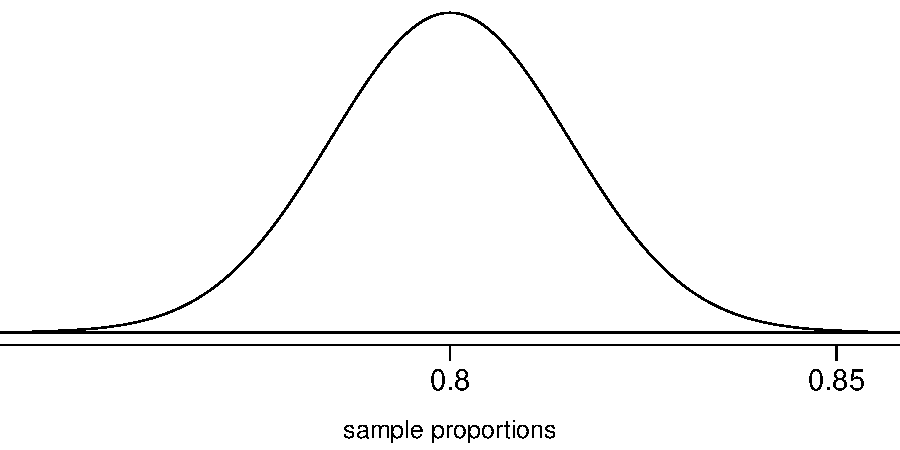
\includegraphics[width=\textwidth]{6-1_single_prop/figures/expdesgn_norm}
\end{center}
}
\pause
Since the p-value is low, we reject $H_0$. The data provide convincing evidence that more than 80\% of Americans have a good intuition on experimental design.

\end{frame}

%%%%%%%%%%%%%%%%%%%%%%%%%%%%%%%%%%%

\subsection{Recap}

%%%%%%%%%%%%%%%%%%%%%%%%%%%%%%%%%%%

\begin{frame}
\frametitle{}

\pq{11\% of 1,001 Americans responding to a 2006 Gallup survey stated that they have objections to celebrating Halloween on religious grounds. At 95\% confidence level, the margin of error for this survey is $\pm 3\%$. A news piece on this study's findings states: ``More than 10\% of all Americans have objections on religious grounds to celebrating Halloween." At 95\% confidence level, is this news piece's statement justified?}

\begin{enumerate}[(a)]
\item Yes
\solnMult{No}
\item Cannot tell
\end{enumerate}

\end{frame}

%%%%%%%%%%%%%%%%%%%%%%%%%%%%%%%%%%

\begin{frame}
\frametitle{Recap - inference for one proportion}

\begin{itemize}

\item Population parameter: $p$, point estimate: $\hat{p}$

\pause

\item Conditions:
\begin{itemize}
\item independence \\
- random sample and 10\% condition
\item at least 10 successes and failures\\ - if not $\rightarrow$ randomization
\end{itemize}

\pause

\item Standard error: $SE = \sqrt{ \frac{p(1-p)}{n} }$
\begin{itemize}
\item for CI: use $\hat{p}$
\item for HT: use $p_0$
\end{itemize}

\end{itemize}

\end{frame}
%%%%%%%%%%%%%%%%%%%%%%%%%%%%%%%%%%%%

\section{Difference of two proportions}

%%%%%%%%%%%%%%%%%%%%%%%%%%%%%%%%%%%%

\begin{frame}
\frametitle{Melting ice cap}

\pq{Scientists predict that global warming may have big effects on the polar regions within the next 100 years. One of the possible effects is that the northern ice cap may completely melt. Would this bother you a great deal, some, a little, or not at all if it actually happened?}

\begin{enumerate}[(a)]
\item A great deal
\item Some
\item A little
\item Not at all
\end{enumerate}

\end{frame}

%%%%%%%%%%%%%%%%%%%%%%%%%%%%%%%%%%%

\begin{frame}
\frametitle{Results from the GSS}

The GSS asks the same question, below are the distributions of responses from the 2010 GSS as well as from a group of introductory statistics students at Duke University: \\

\begin{center}
\begin{tabular}{l r r}
\hline
				& GSS	& Duke \\
\hline
A great deal		& 454	& 69 \\
Some			& 124 	& 30\\
A little			& 52 		& 4\\
Not at all			& 50 		& 2 \\
\hline
Total				& 680 	& 105\\
\hline
\end{tabular}
\end{center}

\end{frame}

%%%%%%%%%%%%%%%%%%%%%%%%%%%%%%%%%%

\begin{frame}
\frametitle{Parameter and point estimate}

\begin{itemize}

\item \hl{Parameter of interest:} Difference between the proportions of \orange{all} Duke students and \orange{all} Americans who would be bothered a great deal by the northern ice cap completely melting.
\[ \mathhl{ p_{Duke} - p_{US} }\]

\pause

\item \hl{Point estimate:} Difference between the proportions of \orange{sampled} Duke students and \orange{sampled} Americans who would be bothered a great deal by the northern ice cap completely melting.
\[ \mathhl{ \hat{p}_{Duke} - \hat{p}_{US} }\]

\end{itemize}

\end{frame}

%%%%%%%%%%%%%%%%%%%%%%%%%%%%%%%%%%%

\begin{frame}
\frametitle{Inference for comparing proportions}

\begin{itemize}

\item The details are the same as before...

\pause

\item CI: \textcolor{orange}{$point~estimate \pm margin~of~error$}

\pause

\item HT: Use \textcolor{orange}{$Z = \frac{point~estimate - null~value}{SE}$} to find appropriate p-value.

\pause

\item We just need the appropriate standard error of the point estimate ($SE_{ \hat{p}_{Duke} - \hat{p}_{US}}$), which is the only new concept.

\end{itemize}

\pause

\formula{Standard error of the difference between two sample proportions}
{
\[ SE_{(\hat{p}_1 - \hat{p}_2)} = \sqrt{ \frac{p_1(1-p_1)}{n_1} + \frac{p_2(1-p_2)}{n_2} } \]
}

\end{frame}

%%%%%%%%%%%%%%%%%%%%%%%%%%%%%%%%%%%%%

\subsection{Confidence intervals for difference of proportions}

%%%%%%%%%%%%%%%%%%%%%%%%%%%%%%%%%%%%%

\begin{frame}
\frametitle{Conditions for CI for difference of proportions}

\begin{enumerate}

\item \hl{Independence within groups: }
\begin{itemize}
\item The US group is sampled randomly and we're assuming that the Duke group represents a random sample as well.
\pause
\item $n_{Duke}$ $<$ 10\% of all Duke students and 680 $<$ 10\% of all Americans.
\end{itemize}
\pause
We can assume that the attitudes of Duke students in the sample are independent of each other, and attitudes of US residents in the sample are independent of each other as well.

\pause

\item \hl{Independence between groups: }
The sampled Duke students and the US residents are independent of each other.

\pause

\item \hl{Success-failure:} \\
At least 10 observed successes and 10 observed failures in the two groups.

\end{enumerate}

\end{frame}

%%%%%%%%%%%%%%%%%%%%%%%%%%%%%%%%%%%%%

\begin{frame}
\frametitle{}

\dq{Construct a 95\% confidence interval for the difference between the proportions of Duke students and Americans who would be bothered a great deal by the melting of the northern ice cap \orange{($p_{Duke} - p_{US}$)}.}

{\footnotesize
\begin{center}
\begin{tabular}{l | c c}
Data			& Duke		& US \\
\hline
A great deal	& 69			& 454 \\
Not a great deal& 36			& 226 \\
\hline
Total			& 105		& 680 \\
\hline
\pause
$\hat{p}$		& 0.657		& 0.668
\end{tabular}
\end{center}
}

\pause

\soln{
\begin{eqnarray*}
&& (\hat{p}_{Duke} - \hat{p}_{US}) \pm z^\star \times \sqrt{ \frac{ \hat{p}_{Duke} (1 - \hat{p}_{Duke})}{n_{Duke} } + \frac{ \hat{p}_{US} (1 -  \hat{p}_{US})}{n_{US} } }  \\
\pause
&=& (0.657 - 0.668) \pause \pm 1.96 \pause \times \sqrt{ \frac{0.657 \times 0.343}{105} + \frac{0.668 \times 0.332}{680} } \\
\pause
&=& -0.011 \pm \pause 1.96 \times 0.0497 \\
\pause
&=& -0.011 \pm 0.097 \\
\pause
&=& (-0.108, 0.086)
\end{eqnarray*}
}


\end{frame}

%%%%%%%%%%%%%%%%%%%%%%%%%%%%%%%%%%%%%

\subsection{HT for comparing proportions}

%%%%%%%%%%%%%%%%%%%%%%%%%%%%%%%%%%%%%

\begin{frame}

\pq{Which of the following is the correct set of hypotheses for testing if the proportion of all Duke students who would be bothered a great deal by the melting of the northern ice cap differs from the proportion of all Americans who do?}

\begin{enumerate}[(a)]
\solnMult{ $H_0:  p_{Duke} = p_{US}$ \\
$H_A:  p_{Duke} \ne p_{US}$ }
\item $H_0:  \hat{p}_{Duke} = \hat{p}_{US}$ \\
$H_A:  \hat{p}_{Duke} \ne \hat{p}_{US}$
\solnMult{ $H_0:  p_{Duke} - p_{US} = 0$ \\
$H_A:  p_{Duke} - p_{US} \ne 0$ }
\item $H_0:  p_{Duke} = p_{US}$ \\
$H_A:  p_{Duke} < p_{US}$
\end{enumerate}

\soln{
\only<2>{\orange{Both (a) and (c) are correct.}}
}

\end{frame}

%%%%%%%%%%%%%%%%%%%%%%%%%%%%%%%%%%

\begin{frame}
\frametitle{Flashback to working with one proportion}

\begin{itemize}

\item When constructing a confidence interval for a population proportion, we check if the \orange{observed} number of successes and failures are at least 10.
\[ n\hat{p} \ge 10 \qquad \qquad n(1-\hat{p}) \ge 10 \]

\pause

\item When conducting a hypothesis test for a population proportion, we check if the \orange{expected} number of successes and failures are at least 10.
\[ np_0 \ge 10 \qquad \qquad n(1-p_0) \ge 10 \]

\end{itemize}

\end{frame}

%%%%%%%%%%%%%%%%%%%%%%%%%%%%%%%%%%%

\begin{frame}
\frametitle{Pooled estimate of a proportion}

\begin{itemize}

\item In the case of comparing two proportions where $H_0: p_1 = p_2$, there isn't a given null value we can use to calculated the \orange{expected} number of successes and failures in each sample.

\pause

\item Therefore, we need to first find a common (\hl{pooled}) proportion for the two groups, and use that in our analysis.

\pause

\item This simply means finding the proportion of total successes among the total number of observations.

\end{itemize}

$\:$ \\

\formula{Pooled estimate of a proportion}
{ \[ \hat{p} = \frac{\#~of~successes_1 + \#~of~successes_2}{n_1 + n_2} \] }

\end{frame}

%%%%%%%%%%%%%%%%%%%%%%%%%%%%%%%%%%%

\begin{frame}
\frametitle{}

\dq{Calculate the estimated \underline{pooled proportion} of Duke students and Americans who would be bothered a great deal by the melting of the northern ice cap. Which sample proportion ($\hat{p}_{Duke}$ or $\hat{p}_{US}$) the pooled estimate is closer to? Why?}

{\footnotesize
\begin{center}
\begin{tabular}{l | c c}
Data			& Duke		& US \\
\hline
A great deal	& 69			& 454 \\
Not a great deal& 36			& 226 \\
\hline
Total			& 105		& 680 \\
\hline
$\hat{p}$		& 0.657		& 0.668
\end{tabular}
\end{center}
}

\pause

\soln{
\begin{eqnarray*}
\hat{p} &=& \frac{\#~of~successes_1 + \#~of~successes_2}{n_1 + n_2} \\
\pause
&=& \frac{69+454}{105+680} \pause = \frac{523}{785} \pause = 0.666
\end{eqnarray*}
}

\end{frame}
%%%%%%%%%%%%%%%%%%%%%%%%%%%%%%%%%%%

\begin{frame}
\frametitle{}

\dq{Do these data suggest that the proportion of all Duke students who would be bothered a great deal by the melting of the northern ice cap differs from the proportion of all Americans who do? Calculate the test statistic, the p-value, and interpret your conclusion in context of the data.}

{\footnotesize
\begin{center}
\begin{tabular}{l | c c}
Data			& Duke		& US \\
\hline
A great deal	& 69			& 454 \\
Not a great deal& 36			& 226 \\
\hline
Total			& 105		& 680 \\
\hline
$\hat{p}$		& 0.657		& 0.668
\end{tabular}
\end{center}
}

\pause

\soln{
\begin{eqnarray*}
Z &=& \frac{(\hat{p}_{Duke} - \hat{p}_{US})}{\sqrt{ \frac{ \hat{p} (1 - \hat{p})}{n_{Duke} } + \frac{ \hat{p} (1 -  \hat{p})}{n_{US} } }} \\
\pause 
&=& \frac{(0.657 - 0.668)}{\sqrt{ \frac{0.666 \times 0.334}{105} + \frac{0.666 \times 0.334}{680} }} = \pause \frac{-0.011}{0.0495} \pause = -0.22 \\
\pause
p-value &=& 2 \times P(Z < -0.22) \pause = 2 \times 0.41 = 0.82
\end{eqnarray*}
}

\end{frame}

%%%%%%%%%%%%%%%%%%%%%%%%%%%%%%%%%%%

\subsection{Recap}

%%%%%%%%%%%%%%%%%%%%%%%%%%%%%%%%%%%

\begin{frame}
\frametitle{Recap - comparing two proportions}

\begin{itemize}

\item Population parameter: $(p_1 - p_2)$, point estimate: $(\hat{p}_1 - \hat{p}_2)$

\pause

\item Conditions:
\pause
\begin{itemize}
\item independence within groups \\
- random sample and 10\% condition met for both groups
\item independence between groups
\item at least 10 successes and failures in each group\\ 
- if not $\rightarrow$ randomization (Section 6.4)
\end{itemize}

\pause

\item $SE_{(\hat{p}_1 - \hat{p}_2)} = \sqrt{ \frac{p_1(1-p_1)}{n_1} + \frac{p_2(1-p_2)}{n_2} }$
\begin{itemize}
\item for CI: use $\hat{p}_1$ and $\hat{p}_2$
\item for HT:
\begin{itemize}
\item when $H_0: p_1 = p_2$: use $\hat{p}_{pool} = \frac{\#~suc_1 + \#suc_2}{n_1 + n_2}$
\item when $H_0: p_1 - p_2 = $ \textit{(some value other than 0)}: use $\hat{p}_1$ and $\hat{p}_2$ \\
- this is pretty rare
\end{itemize}
\end{itemize}

\end{itemize}

\end{frame}

%%%%%%%%%%%%%%%%%%%%%%%%%%%%%%%%%%%

\begin{frame}
\frametitle{Reference - standard error calculations}

\begin{center}
\begin{tabular}{l | l | l}
			& one sample					& two samples \\ 
\hline
& & \\
mean		& $SE = \frac{s}{\sqrt{n}}$			& $SE = \sqrt{ \frac{s_1^2}{n_1} + \frac{s_2^2}{n_2}}$ \\
& & \\
\hline
& & \\
proportion		& $SE = \sqrt{ \frac{p(1-p)}{n} }$	& $SE = \sqrt{ \frac{p_1(1-p_1)}{n_1} + \frac{p_2(1-p_2)}{n_2} }$	 \\	
& & \\
\end{tabular}
\end{center}

\pause

\begin{itemize}

\item When working with means, it's very rare that $\sigma$ is known, so we usually use $s$.

\pause

\item When working with proportions, 
\begin{itemize}
\item if doing a hypothesis test, $p$ comes from the null hypothesis
\item if constructing a confidence interval, use $\hat{p}$ instead
\end{itemize}

\end{itemize}

\end{frame}
%%%%%%%%%%%%%%%%%%%%%%%%%%%%%%%%%%%%

\section{Chi-square test of GOF}

%%%%%%%%%%%%%%%%%%%%%%%%%%%%%%%%%%%

\subsection{Weldon's dice}

%%%%%%%%%%%%%%%%%%%%%%%%%%%%%%%%%%%

\begin{frame}
\frametitle{Weldon's dice}

\twocol{0.7}{0.3}
{
\begin{itemize}

\item Walter Frank Raphael Weldon (1860 - 1906), was an English evolutionary biologist and a founder of biometry. He was the joint founding editor of Biometrika, with Francis Galton and Karl Pearson.

\item In 1894, he rolled 12 dice 26,306 times, and recorded the number of 5s or 6s (which he considered to be a success).

\end{itemize}
}
{
\begin{center}
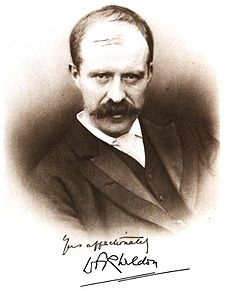
\includegraphics[width=\textwidth]{6-3_chisq_gof/figures/dice/weldon}
\end{center}
}
\begin{itemize}

\item It was observed that 5s or 6s occurred more often than expected, and Pearson hypothesized that this was probably due to the construction of the dice. Most inexpensive dice have hollowed-out pips, and since opposite sides add to 7, the face with 6 pips is lighter than its opposing face, which has only 1 pip.

\end{itemize}

\end{frame}

%%%%%%%%%%%%%%%%%%%%%%%%%%%%%%%%%%%

\begin{frame}
\frametitle{Labby's dice}

\twocol{0.5}{0.5}
{
\begin{itemize}

\item In 2009, Zacariah Labby (U of Chicago), repeated Weldon's experiment using a homemade dice-throwing, pip counting machine.
\begin{center}
\webURL{http://www.youtube.com/watch?v=95EErdouO2w}
\end{center}

\item The rolling-imaging process took about 20 seconds per roll.

\end{itemize}
}
{
\begin{center}
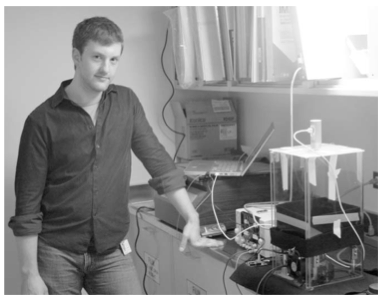
\includegraphics[width=\textwidth]{6-3_chisq_gof/figures/dice/labby}
\end{center}
}

\begin{itemize}

\item Each day there were $\sim$150 images to process manually.

\item At this rate Weldon's experiment was repeated in a little more than six full days.

\item Recommended reading: \webURL{http://galton.uchicago.edu/about/docs/labby09dice.pdf}

\end{itemize}

\end{frame}

%%%%%%%%%%%%%%%%%%%%%%%%%%%%%%%%%%%

\begin{frame}
\frametitle{Labby's dice (cont.)}

\begin{itemize}

\item Labby did not actually observe the same phenomenon that Weldon observed (higher frequency of 5s and 6s).

\item Automation allowed Labby to collect more data than Weldon did in 1894, instead of recording ``successes" and ``failures", Labby recorded the individual number of pips on each die.

\end{itemize}

\begin{center}
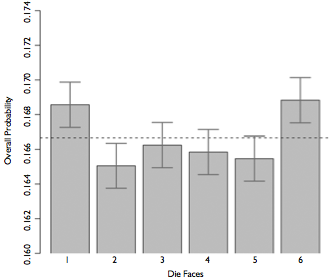
\includegraphics[width=0.55\textwidth]{6-3_chisq_gof/figures/dice/labbyPipCounts}
\end{center}

\end{frame}

%%%%%%%%%%%%%%%%%%%%%%%%%%%%%%%%%%%

\subsection*{Creating a test statistic for one-way tables}

%%%%%%%%%%%%%%%%%%%%%%%%%%%%%%%%%%%

\begin{frame}
\frametitle{Expected counts}

\pq{Labby rolled 12 dice 26,306 times. If each side is equally likely to come up, how many 1s, 2s, $\cdots$, 6s would he expect to have observed?}

\begin{enumerate}[(a)]
\item $\frac{1}{6}$
\item $\frac{12}{6}$
\item $\frac{26,306}{6}$
\solnMult{ $\frac{12 \times 26,306}{6}$ } \soln{\only<2>{\orange{$= 52,612$}}}
\end{enumerate}

\end{frame}

%%%%%%%%%%%%%%%%%%%%%%%%%%%%%%%%%%%

\begin{frame}
\frametitle{Summarizing Labby's results}

The table below shows the observed and expected counts from Labby's experiment.

{\small
\begin{center}
\renewcommand\arraystretch{1.25}
\begin{tabular}{c | c c}
Outcome	& Observed	& Expected \\
\hline
1		& 53,222		& 52,612 \\
2		& 52,118		& 52,612 \\
3		& 52,465		& 52,612 \\
4		& 52,338		& 52,612 \\
5		& 52,244		& 52,612 \\
6		& 53,285		& 52,612 \\
\hline
Total		& 315,672		& 315,672
\end{tabular}
\end{center}
}

\pause
\dq{Why are the expected counts the same for all outcomes but the observed counts are different? At a first glance, does there appear to be an inconsistency between the observed and expected counts?}

\end{frame}

%%%%%%%%%%%%%%%%%%%%%%%%%%%%%%%%%%%

\begin{frame}
\frametitle{Setting the hypotheses}

\dq{Do these data provide convincing evidence of an inconsistency between the observed and expected counts?}

\pause

\begin{itemize}
\item[$H_0$:] There is no inconsistency between the observed and the expected counts. \hlGr{The observed counts follow the same distribution as the expected counts.}

\pause

\item[$H_A$:] There is an inconsistency between the observed and the expected counts. \hlGr{The observed counts \orange{do not} follow the same distribution as the expected counts.} There is a bias in which side comes up on the roll of a die.
\end{itemize}

\end{frame}

%%%%%%%%%%%%%%%%%%%%%%%%%%%%%%%%%%%

\begin{frame}
\frametitle{Evaluating the hypotheses}

\begin{itemize}

\item To evaluate these hypotheses, we quantify how different the observed counts are from the expected counts. 

\pause

\item Large deviations from what would be expected based on sampling variation (chance) alone provide strong evidence for the alternative hypothesis.

\pause

\item This is called a \hl{goodness of fit} test since we're evaluating how well the observed data fit the expected distribution.

\end{itemize}

\end{frame}

%%%%%%%%%%%%%%%%%%%%%%%%%%%%%%%%%%%

\subsection{The chi-square test statistic}

%%%%%%%%%%%%%%%%%%%%%%%%%%%%%%%%%%%

\begin{frame}
\frametitle{Anatomy of a test statistic}

\begin{itemize}

\item The general form of a test statistic is
\[ \frac{\text{point estimate} - \text{null value}}{\text{SE of point estimate}} \]

\pause

\item This construction is based on 
\begin{enumerate}
\item identifying the difference between a point estimate and an expected value if the null hypothesis was true, and 
\item standardizing that difference using the standard error of the point estimate. 
\end{enumerate}
\pause

These two ideas will help in the construction of an appropriate test statistic for count data.

\end{itemize}

\end{frame}

%%%%%%%%%%%%%%%%%%%%%%%%%%%%%%%%%%%

\begin{frame}
\frametitle{Chi-square statistic}

When dealing with counts and investigating how far the observed counts are from the expected counts, we use a new test statistic called the \hl{chi-square ($\chi^2$) statistic}.

$\:$ \\

\pause

\formula{$\chi^2$ statistic}
{
\[\chi^2 = \sum_{i = 1}^k \frac{(O - E)^2}{E} \qquad \text{where $k$ = total number of cells} \]
}

\end{frame}

%%%%%%%%%%%%%%%%%%%%%%%%%%%%%%%%%%%

\begin{frame}
\frametitle{Calculating the chi-square statistic}

\begin{center}
\renewcommand\arraystretch{1.8}
\begin{tabular}{c | c c | c}
Outcome	& Observed	& Expected 	& $\frac{(O - E)^2}{E}$\\
\hline
1		& 53,222		& 52,612 		& $\frac{(53,222 - 52,612)^2}{52,612} = 7.07$ \\
\pause
2		& 52,118		& 52,612 		& $\frac{(52,118 - 52,612)^2}{52,612} = 4.64$ \\
\pause
3		& 52,465		& 52,612 		& $\frac{(52,465 - 52,612)^2}{52,612} = 0.41$ \\
\pause
4		& 52,338		& 52,612 		& $\frac{(52,338 - 52,612)^2}{52,612} = 1.43$\\
\pause
5		& 52,244		& 52,612 		& $\frac{(52,244 - 52,612)^2}{52,612} = 2.57$\\
\pause
6		& 53,285		& 52,612 		& $\frac{(53,285 - 52,612)^2}{52,612} = 8.61$\ \\
\hline
\pause
Total		& 315,672		& 315,672		& 24.73
\end{tabular}
\end{center}

\end{frame}

%%%%%%%%%%%%%%%%%%%%%%%%%%%%%%%%%%%

\begin{frame}
\frametitle{Why square?}


Squaring the difference between the observed and the expected outcome does two things:
\pause
\begin{itemize}
\item Any standardized difference that is squared will now be positive.
\pause
\item Differences that already looked unusual will become much larger after being squared.
\end{itemize}

\vspace{1cm}

\pause
\dq{When have we seen this before?}

\end{frame}

%%%%%%%%%%%%%%%%%%%%%%%%%%%%%%%%%%%

\subsection{The chi-square distribution and finding areas}

%%%%%%%%%%%%%%%%%%%%%%%%%%%%%%%%%%%

\begin{frame}
\frametitle{The chi-square distribution}

\begin{itemize}

\item In order to determine if the $\chi^2$ statistic we calculated is considered unusually high or not we need to first describe its distribution.

\pause

\item The chi-square distribution has just one parameter called \hl{degrees of freedom (df)}, which influences the shape, center, and spread of the distribution. \\

\end{itemize}

\pause

$\:$ \\

\Remember{So far we've seen three other continuous distributions:
\begin{itemize}
\item[-] normal distribution: unimodal and symmetric with two parameters: mean and standard deviation
\item[-] T distribution: unimodal and symmetric with one parameter: degrees of freedom
\item[-] F distribution: unimodal and right skewed with two parameters: degrees of freedom or numerator (between group variance) and denominator (within group variance)
\end{itemize}
}

\end{frame}

%%%%%%%%%%%%%%%%%%%%%%%%%%%%%%%%%%%

\begin{frame}
\frametitle{}

\pq{Which of the following is false?}

\begin{center}
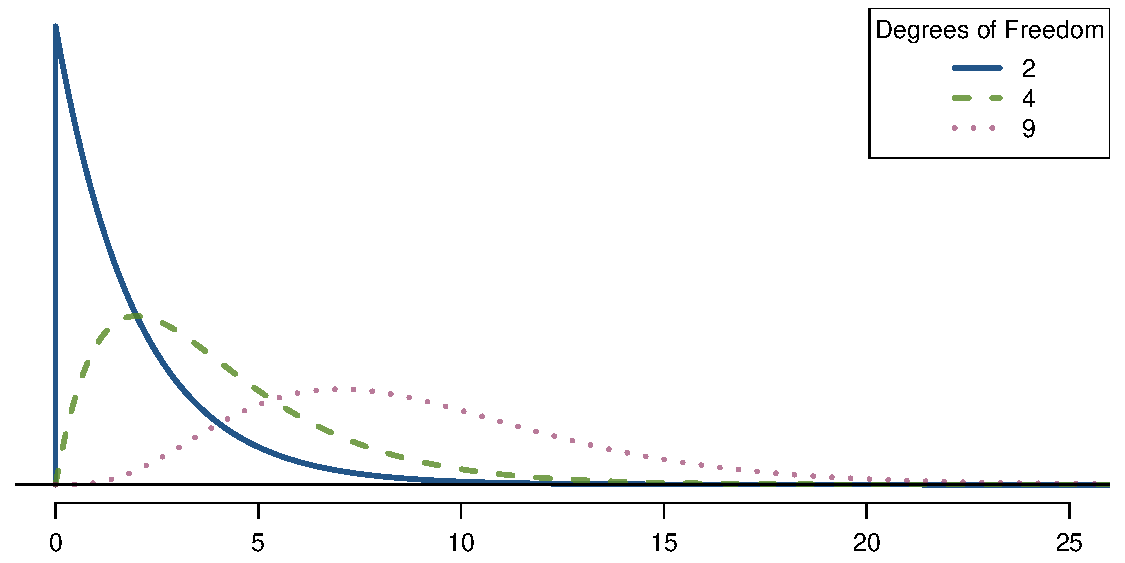
\includegraphics[width=0.7\textwidth]{6-3_chisq_gof/figures/chiSquareDistributionWithInceasingDF/chiSquareDistributionWithInceasingDF}
\end{center}

As the df increases,
\begin{enumerate}[(a)]
\item the center of the $\chi^2$ distribution increases as well
\item the variability of the $\chi^2$ distribution increases as well
\solnMult{the shape of the $\chi^2$ distribution becomes more skewed (less like a normal)}
\end{enumerate}

\end{frame}

%%%%%%%%%%%%%%%%%%%%%%%%%%%%%%%%%%%

\begin{frame}[fragile]
\frametitle{Finding areas under the chi-square curve}

\begin{itemize}

\item p-value = tail area under the chi-square distribution (as usual)

\pause

\item For this we can use technology, or a \hl{chi-square probability table}.

\pause

\item  This table works a lot like the $t$ table, but only provides upper tail values.
\end{itemize}

\begin{center}
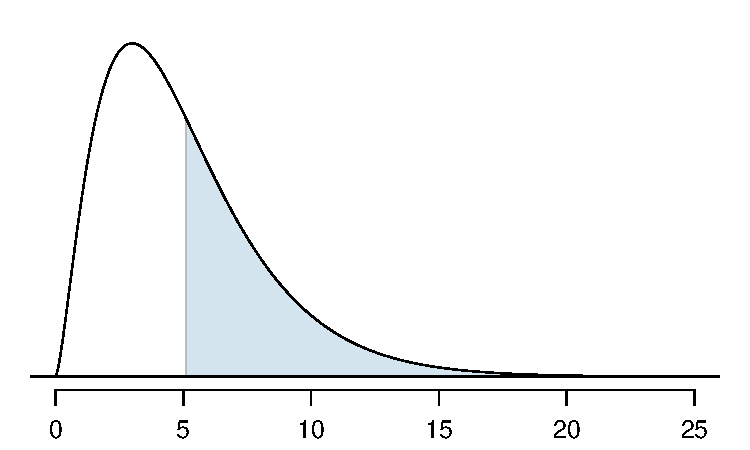
\includegraphics[width=0.3\textwidth]{6-3_chisq_gof/figures/above5Point1WithDF5/above5Point1WithDF5}
\end{center}

{\scriptsize
\begin{center}
\begin{tabular}{r | rrrr | rrrr |}
  \hline
Upper tail & 0.3 & 0.2 & 0.1 & 0.05 & 0.02 & 0.01 & 0.005 & 0.001 \\ 
  \hline
df \hfill 1 &  1.07 &  1.64 &  2.71 &  3.84 &  5.41 &  6.63 &  7.88 &  10.83 \\ 
  2 &  2.41 &  3.22 &  4.61 &  5.99 &  7.82 &  9.21 &  10.60 &  13.82 \\ 
  3 &  3.66 &  4.64 &  6.25 &  7.81 &  9.84 &  11.34 &  12.84 &  16.27 \\ 
  4 &  4.88 &  5.99 &  7.78 &  9.49 &  11.67 &  13.28 &  14.86 &  18.47 \\ 
  5 &  6.06 &  7.29 &  9.24 &  11.07 &  13.39 &  15.09 &  16.75 &  20.52 \\ 
  \hline
  6 &  7.23 &  8.56 &  10.64 &  12.59 &  15.03 &  16.81 &  18.55 &  22.46 \\ 
  7 &  8.38 &  9.80 &  12.02 &  14.07 &  16.62 &  18.48 &  20.28 &  24.32 \\ 
  $\cdots$ &   &   &   &   &   &   &   &   \\ 
\end{tabular}
\end{center}
}

\end{frame}

%%%%%%%%%%%%%%%%%%%%%%%%%%%%%%%%%%%

\begin{frame}
\frametitle{Finding areas under the chi-square curve (cont.)}

\dq{Estimate the shaded area under the chi-square curve with $df = 6$.}

\twocol{0.6}{0.4}{
\begin{center}
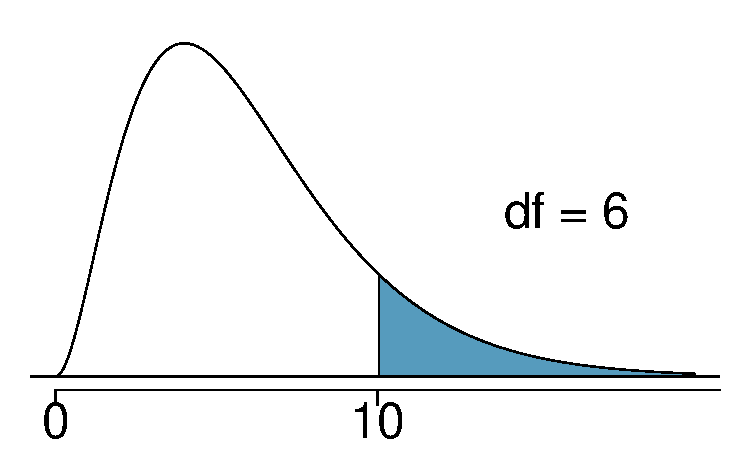
\includegraphics[width=0.67\textwidth]{6-3_chisq_gof/figures/above10WithDF6/above10WithDF6}
\end{center}
}
{\only<4 |handout:0>{\orange{$P(\chi^2_{df = 6} > 10)$\\ is between 0.1 and 0.2}}
}

\only<1>{
\begin{center}
{\footnotesize
\begin{tabular}{r | rrrr | rrrr |}
  \hline
Upper tail & 0.3 & 0.2 & 0.1 & 0.05 & 0.02 & 0.01 & 0.005 & 0.001 \\ 
  \hline
df \hfill 1 &  1.07 &  1.64 &  2.71 &  3.84 &  5.41 &  6.63 &  7.88 &  10.83 \\ 
  2 &  2.41 &  3.22 &  4.61 &  5.99 &  7.82 &  9.21 &  10.60 &  13.82 \\ 
  3 &  3.66 &  4.64 &  6.25 &  7.81 &  9.84 &  11.34 &  12.84 &  16.27 \\ 
  4 &  4.88 &  5.99 &  7.78 &  9.49 &  11.67 &  13.28 &  14.86 &  18.47 \\ 
  5 &  6.06 &  7.29 &  9.24 &  11.07 &  13.39 &  15.09 &  16.75 &  20.52 \\ 
  \hline
  6 &  7.23 &  8.56 &   10.64  &  12.59 &  15.03 &  16.81 &  18.55 &  22.46 \\ 
  7 &  8.38 &  9.80 &  12.02 &  14.07 &  16.62 &  18.48 &  20.28 &  24.32 \\ 
  \hline
\end{tabular}
}
\end{center}
}

\only<2 | handout:0>{
\begin{center}
{\footnotesize
\begin{tabular}{r | rrrr | rrrr |}
  \hline
Upper tail & 0.3 & 0.2 & 0.1 & 0.05 & 0.02 & 0.01 & 0.005 & 0.001 \\ 
  \hline
df \hfill 1 &  1.07 &  1.64 &  2.71 &  3.84 &  5.41 &  6.63 &  7.88 &  10.83 \\ 
  2 &  2.41 &  3.22 &  4.61 &  5.99 &  7.82 &  9.21 &  10.60 &  13.82 \\ 
  3 &  3.66 &  4.64 &  6.25 &  7.81 &  9.84 &  11.34 &  12.84 &  16.27 \\ 
  4 &  4.88 &  5.99 &  7.78 &  9.49 &  11.67 &  13.28 &  14.86 &  18.47 \\ 
  5 &  6.06 &  7.29 &  9.24 &  11.07 &  13.39 &  15.09 &  16.75 &  20.52 \\ 
  \hline
\rowcolor[gray]{.6}
  6 &  7.23 &  8.56 &   10.64  &  12.59 &  15.03 &  16.81 &  18.55 &  22.46 \\ 
  7 &  8.38 &  9.80 &  12.02 &  14.07 &  16.62 &  18.48 &  20.28 &  24.32 \\ 
  \hline
\end{tabular}
}
\end{center}
}

\only<3 | handout:0>{
\begin{center}
{\footnotesize
\begin{tabular}{r | rrrr | rrrr |}
  \hline
Upper tail & 0.3 & 0.2 & 0.1 & 0.05 & 0.02 & 0.01 & 0.005 & 0.001 \\ 
  \hline
df \hfill 1 &  1.07 &  1.64 &  2.71 &  3.84 &  5.41 &  6.63 &  7.88 &  10.83 \\ 
  2 &  2.41 &  3.22 &  4.61 &  5.99 &  7.82 &  9.21 &  10.60 &  13.82 \\ 
  3 &  3.66 &  4.64 &  6.25 &  7.81 &  9.84 &  11.34 &  12.84 &  16.27 \\ 
  4 &  4.88 &  5.99 &  7.78 &  9.49 &  11.67 &  13.28 &  14.86 &  18.47 \\ 
  5 &  6.06 &  7.29 &  9.24 &  11.07 &  13.39 &  15.09 &  16.75 &  20.52 \\ 
  \hline
  \rowcolor[gray]{.6}
  6 &  7.23 & \orange{ 8.56 }&  \orange{ 10.64 } &  12.59 &  15.03 &  16.81 &  18.55 &  22.46 \\ 
  7 &  8.38 &  9.80 &  12.02 &  14.07 &  16.62 &  18.48 &  20.28 &  24.32 \\ 
  \hline
\end{tabular}
}
\end{center}
}

\only<4 | handout:0>{
\begin{center}
{\footnotesize
\begin{tabular}{r | r >{\columncolor[gray]{0.6}[.5\tabcolsep]}r >{\columncolor[gray]{0.6}[.5\tabcolsep]}rr | rrrr |}
  \hline
Upper tail & 0.3 & \orange{0.2} & \orange{0.1} & 0.05 & 0.02 & 0.01 & 0.005 & 0.001 \\ 
  \hline
df \hfill 1 &  1.07 &  1.64 &  2.71 &  3.84 &  5.41 &  6.63 &  7.88 &  10.83 \\ 
  2 &  2.41 &  3.22 &  4.61 &  5.99 &  7.82 &  9.21 &  10.60 &  13.82 \\ 
  3 &  3.66 &  4.64 &  6.25 &  7.81 &  9.84 &  11.34 &  12.84 &  16.27 \\ 
  4 &  4.88 &  5.99 &  7.78 &  9.49 &  11.67 &  13.28 &  14.86 &  18.47 \\ 
  5 &  6.06 &  7.29 &  9.24 &  11.07 &  13.39 &  15.09 &  16.75 &  20.52 \\ 
  \hline
  \rowcolor[gray]{.6}
  6 &  7.23 & \orange{ 8.56 }&  \orange{ 10.64 } &  12.59 &  15.03 &  16.81 &  18.55 &  22.46 \\ 
  7 &  8.38 &  9.80 &  12.02 &  14.07 &  16.62 &  18.48 &  20.28 &  24.32 \\ 
  \hline
\end{tabular}
}
\end{center}
}

\end{frame}

%%%%%%%%%%%%%%%%%%%%%%%%%%%%%%%%%%%

\begin{frame}
\frametitle{Finding areas under the chi-square curve (cont.)}

\pq{Estimate the shaded area (above 17) under the $\chi^2$ curve with $df = 9$.}

\twocol{0.6}{0.4}{
\begin{center}
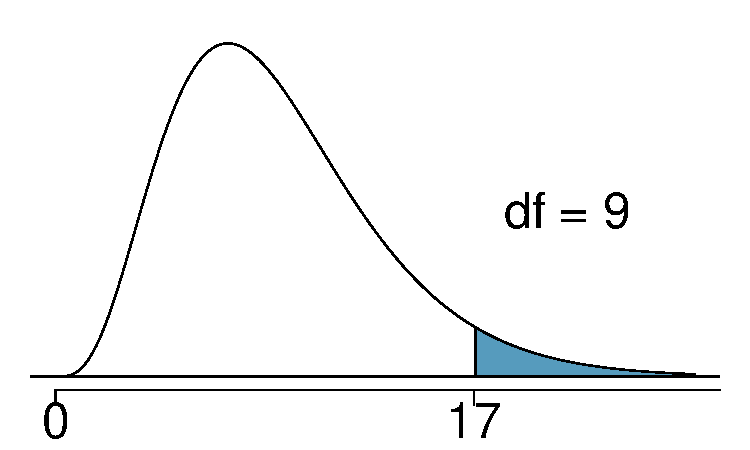
\includegraphics[width=0.67\textwidth]{6-3_chisq_gof/figures/above17WithDF9/above17WithDF9}
\end{center}
}
{
{\small
\begin{enumerate}[(a)]
\setlength{\itemsep}{0in}
\item 0.05
\item 0.02
\solnMult{between 0.02 and 0.05}
\item between 0.05 and 0.1
\item between 0.01 and 0.02
\end{enumerate}
}
}

\only<1>{
\begin{center}
{\scriptsize
\begin{tabular}{r | rrrr | rrrr |}
  \hline
Upper tail & 0.3 & 0.2 & 0.1 & 0.05 & 0.02 & 0.01 & 0.005 & 0.001 \\ 
  \hline
df  \hfill 7 &  8.38 &  9.80 &  12.02 &  14.07 &  16.62 &  18.48 &  20.28 &  24.32 \\ 
  8 &  9.52 &  11.03 &  13.36 &  15.51 &  18.17 &  20.09 &  21.95 &  26.12 \\ 
  9 &  10.66 &  12.24 &  14.68 &  16.92 &  19.68 &  21.67 &  23.59 &  27.88 \\ 
  10 &  11.78 &  13.44 &  15.99 &  18.31 &  21.16 &  23.21 &  25.19 &  29.59 \\ 
  \hline
  11 &   12.90 &  14.63 &  17.28 &  19.68 &  22.62 &  24.72 &  26.76 &  31.26 \\ 
\end{tabular}
}
\end{center}
}

\only<2 | handout:0>{
\begin{center}
{\scriptsize
\begin{tabular}{r | rrr >{\columncolor[gray]{0.6}[.5\tabcolsep]}r | >{\columncolor[gray]{0.6}[.5\tabcolsep]}rrrr |}
  \hline
Upper tail & 0.3 & 0.2 & 0.1 & \orange{ 0.05 } & \orange{ 0.02 } & 0.01 & 0.005 & 0.001 \\ 
  \hline
df  \hfill 7 &  8.38 &  9.80 &  12.02 &  14.07 &  16.62 &  18.48 &  20.28 &  24.32 \\ 
  8 &  9.52 &  11.03 &  13.36 &  15.51 &  18.17 &  20.09 &  21.95 &  26.12 \\ 
    \rowcolor[gray]{.6}
  9 &  10.66 &  12.24 &  14.68 &  \orange{16.92 }&  \orange{19.68} &  21.67 &  23.59 &  27.88 \\ 
  10 &  11.78 &  13.44 &  15.99 &  18.31 &  21.16 &  23.21 &  25.19 &  29.59 \\ 
  \hline
  11 &   12.90 &  14.63 &  17.28 &  19.68 &  22.62 &  24.72 &  26.76 &  31.26 \\ 
  \hline
\end{tabular}
}
\end{center}
}

\end{frame}

%%%%%%%%%%%%%%%%%%%%%%%%%%%%%%%%%%%

\begin{frame}
\frametitle{Finding areas under the chi-square curve (one more)}

\pq{Estimate the shaded area (above 30) under the $\chi^2$ curve with $df = 10$.}

\twocol{0.6}{0.4}{
\begin{center}
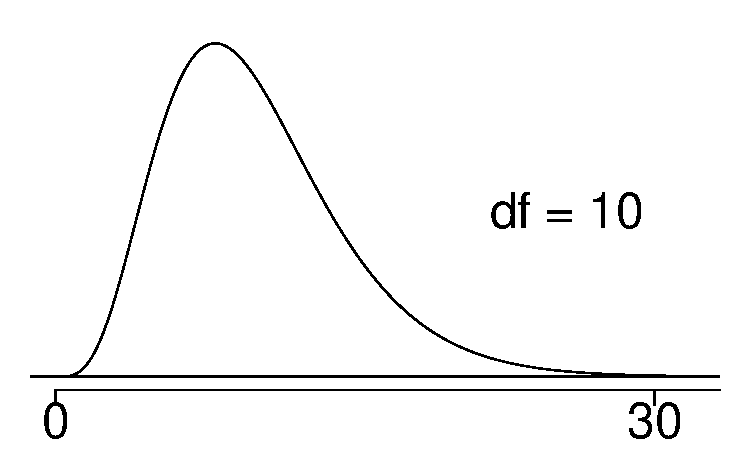
\includegraphics[width=0.67\textwidth]{6-3_chisq_gof/figures/above30WithDF10/above30WithDF10}
\end{center}
}
{
{\small
\begin{enumerate}[(a)]
\setlength{\itemsep}{0in}
\item greater than 0.3
\item between 0.005 and 0.001
\solnMult{less than 0.001}
\item greater than 0.001
\item cannot tell using this table
\end{enumerate}
}
}

\only<1>{
\begin{center}
{\scriptsize
\begin{tabular}{r | rrrr | rrrr |}
  \hline
Upper tail & 0.3 & 0.2 & 0.1 & 0.05 & 0.02 & 0.01 & 0.005 & 0.001 \\ 
  \hline
df  \hfill 7 &  8.38 &  9.80 &  12.02 &  14.07 &  16.62 &  18.48 &  20.28 &  24.32 \\ 
  8 &  9.52 &  11.03 &  13.36 &  15.51 &  18.17 &  20.09 &  21.95 &  26.12 \\ 
  9 &  10.66 &  12.24 &  14.68 &  16.92 &  19.68 &  21.67 &  23.59 &  27.88 \\ 
  10 &  11.78 &  13.44 &  15.99 &  18.31 &  21.16 &  23.21 &  25.19 &  29.59 \\ 
  \hline
  11 &   12.90 &  14.63 &  17.28 &  19.68 &  22.62 &  24.72 &  26.76 &  31.26 \\ 
\end{tabular}
}
\end{center}
}

\only<2 | handout:0>{
\begin{center}
{\scriptsize
\begin{tabular}{r | rrrr | rrr>{\columncolor[gray]{0.6}[.5\tabcolsep]}r | c}
  \cline{1-9}
Upper tail & 0.3 & 0.2 & 0.1 & 0.05 &  0.02  & 0.01 & 0.005 & \orange{0.001} & \mathhl{\rightarrow}  \\ 
  \cline{1-9}
df  \hfill 7 &  8.38 &  9.80 &  12.02 &  14.07 &  16.62 &  18.48 &  20.28 &  24.32 \\ 
  8 &  9.52 &  11.03 &  13.36 &  15.51 &  18.17 &  20.09 &  21.95 &  26.12 \\ 
  9 &  10.66 &  12.24 &  14.68 &  16.92 &  19.68 &  21.67 &  23.59 &  27.88 \\ 
    \rowcolor[gray]{.6}
  10 &  11.78 &  13.44 &  15.99 &  18.31 &  21.16 &  23.21 &  25.19 &  \orange{29.59} & \mathhl{\rightarrow} \\ 
  \cline{1-9}
  11 &   12.90 &  14.63 &  17.28 &  19.68 &  22.62 &  24.72 &  26.76 &  31.26 \\ 
  \cline{1-9}
\end{tabular}
}
\end{center}
}

\end{frame}

%%%%%%%%%%%%%%%%%%%%%%%%%%%%%%%%%%%

\begin{frame}[fragile]
\frametitle{Finding the tail areas using computation}

\begin{itemize}

\item While probability tables are very helpful in understanding how probability distributions work, and provide quick reference when computational resources are not available, they are somewhat archaic.

\pause

\item Using R:
{\footnotesize
\begin{lstlisting}
pchisq(q = 30, df = 10, lower.tail = FALSE)
# 0.0008566412
\end{lstlisting}
}

\pause

\item Using a web applet:

\webURL{http://bitly.com/dist_calc}

\end{itemize}

\end{frame}

%%%%%%%%%%%%%%%%%%%%%%%%%%%%%%%%%%%

\subsection{Finding a p-value for a chi-square test}

%%%%%%%%%%%%%%%%%%%%%%%%%%%%%%%%%%%

\begin{frame}
\frametitle{Back to Labby's dice}

\begin{itemize}

\item The research question was: Do these data provide convincing evidence of an inconsistency between the observed and expected counts?

\pause

\item The hypotheses were:
\begin{itemize}
\item[$H_0$:] There is no inconsistency between the observed and the expected counts. The observed counts follow the same distribution as the expected counts.
\item[$H_A$:] There is an inconsistency between the observed and the expected counts. The observed counts \orange{do not} follow the same distribution as the expected counts. There is a bias in which side comes up on the roll of a die.
\end{itemize}

\pause

\item We had calculated a test statistic of \orange{$\chi^2 = 24.67$}.

\pause

\item All we need is the $df$ and we can calculate the tail area (the p-value) and make a decision on the hypotheses.

\end{itemize}

\end{frame}

%%%%%%%%%%%%%%%%%%%%%%%%%%%%%%%%%%%

\begin{frame}
\frametitle{Degrees of freedom for a goodness of fit test}

\begin{itemize}

\item When conducting a goodness of fit test to evaluate how well the observed data follow an expected distribution, the degrees of freedom are calculated as the number of cells ($k$) minus 1.
\[ \mathhl{df = k - 1} \]

\pause

\item For dice outcomes, $k = 6$, therefore
\[ df = 6 - 1 = 5 \]

\end{itemize}

\end{frame}

%%%%%%%%%%%%%%%%%%%%%%%%%%%%%%%%%%%

\begin{frame}
\frametitle{Finding a p-value for a chi-square test}

The \hl{p-value} for a chi-square test is defined as the \hl{tail area above the calculated test statistic}.

\twocol{0.6}{0.4}{
\begin{center}
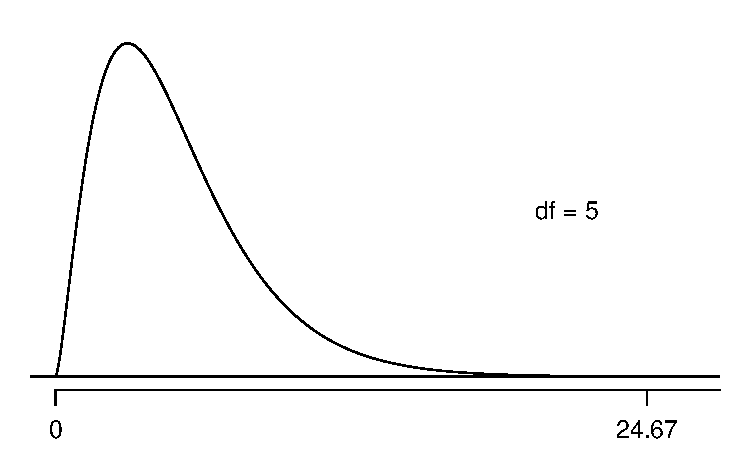
\includegraphics[width=0.67\textwidth]{6-3_chisq_gof/figures/above24Point67WithDF5/above24Point67WithDF5}
\end{center}
}
{
p-value = $P(\chi^2_{df = 5} > 24.67)$\\ is less than 0.001
}

\begin{center}
{\footnotesize
\begin{tabular}{r | rrrr | rrrr r}
  \hline
Upper tail & 0.3 & 0.2 & 0.1 & 0.05 & 0.02 & 0.01 & 0.005 & 0.001 & \orange{$\rightarrow$}  \\ 
  \hline
df \hfill 1 &  1.07 &  1.64 &  2.71 &  3.84 &  5.41 &  6.63 &  7.88 &  10.83 \\ 
  2 &  2.41 &  3.22 &  4.61 &  5.99 &  7.82 &  9.21 &  10.60 &  13.82 \\ 
  3 &  3.66 &  4.64 &  6.25 &  7.81 &  9.84 &  11.34 &  12.84 &  16.27 \\ 
  4 &  4.88 &  5.99 &  7.78 &  9.49 &  11.67 &  13.28 &  14.86 &  18.47 \\ 
  \rowcolor[gray]{.6}
  5 &  6.06 &  7.29 &  9.24 &  11.07 &  13.39 &  15.09 &  16.75 &  20.52 &\orange{$\rightarrow$} \\ 
  \hline
\end{tabular}
}
\end{center}

\end{frame}

%%%%%%%%%%%%%%%%%%%%%%%%%%%%%%%%%%%

\begin{frame}
\frametitle{Conclusion of the hypothesis test}

\pq{We calculated a p-value less than 0.001. At 5\% significance level, what is the conclusion of the hypothesis test?}

\begin{enumerate}[(a)]
\item Reject $H_0$, the data provide convincing evidence that the dice are fair.
\solnMult{Reject $H_0$, the data provide convincing evidence that the dice are biased.}
\item Fail to reject $H_0$, the data provide convincing evidence that the dice are fair.
\item Fail to reject $H_0$, the data provide convincing evidence that the dice are biased.
\end{enumerate}

\end{frame}

%%%%%%%%%%%%%%%%%%%%%%%%%%%%%%%%%%%

\begin{frame}
\frametitle{Turns out...}

\begin{itemize}

\item The 1-6 axis is consistently shorter than the other two (2-5 and 3-4), thereby supporting the hypothesis that the faces with one and six pips are larger than the other faces.

\item Pearson's claim that 5s and 6s appear more often due to the carved-out pips is not supported by these data.

\item Dice used in casinos have flush faces, where the pips are filled in with a plastic of the same density as the surrounding material and are precisely balanced.

\end{itemize}

\begin{center}
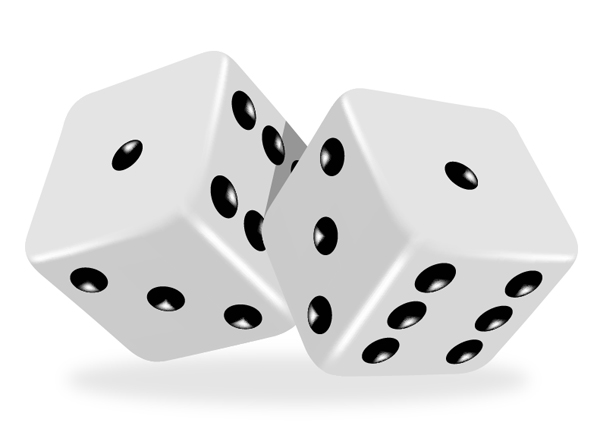
\includegraphics[width=0.3\textwidth]{6-3_chisq_gof/figures/dice/regular}
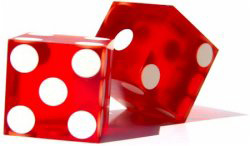
\includegraphics[width=0.3\textwidth]{6-3_chisq_gof/figures/dice/casino}
\end{center}


\end{frame}

%%%%%%%%%%%%%%%%%%%%%%%%%%%%%%%%%%%

\begin{frame}
\frametitle{Recap: p-value for a chi-square test}

\begin{itemize}

\item The p-value for a chi-square test is defined as the tail area \hl{above} the calculated test statistic.

\item This is because the test statistic is always positive, and a higher test statistic means a stronger deviation from the null hypothesis.

\end{itemize}

\begin{center}
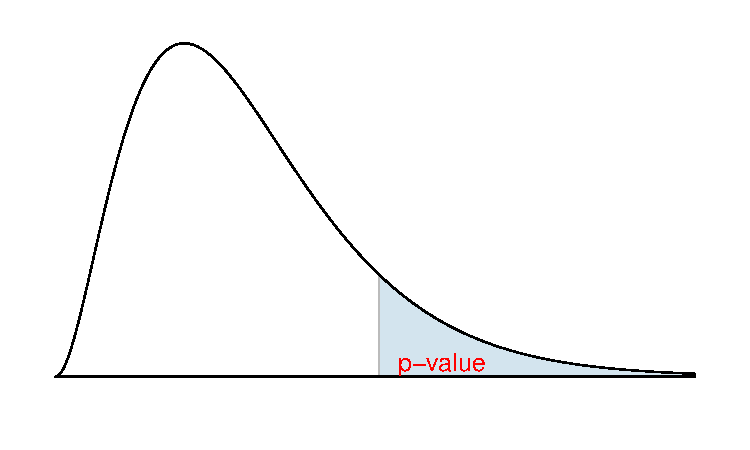
\includegraphics[width=0.7\textwidth]{6-3_chisq_gof/figures/genericChiSquare/genericChiSquare}
\end{center}

\end{frame}

%%%%%%%%%%%%%%%%%%%%%%%%%%%%%%%%%%%

\begin{frame}
\frametitle{Conditions for the chi-square test}

\begin{enumerate}

\item \hlGr{Independence:} Each case that contributes a count to the table must be independent of all the other cases in the table.

\pause

\item \hlGr{Sample size:} Each particular scenario (i.e. cell) must have at least 5 \orange{expected} cases.

\pause

\item \hlGr{df $>$ 1:} Degrees of freedom must be greater than 1.

\end{enumerate}

\pause

Failing to check conditions may unintentionally affect the test's error rates.

\end{frame}

%%%%%%%%%%%%%%%%%%%%%%%%%%%%%%%%%%%

\subsection{2009 Iran Election}

%%%%%%%%%%%%%%%%%%%%%%%%%%%%%%%%%%%

\begin{frame}
\frametitle{2009 Iran Election}

\dq{There was lots of talk of election fraud in the 2009 Iran election. We'll compare the data from a poll conducted before the election (observed data) to the reported votes in the election to see if the two follow the same distribution.}

\begin{center}
\begin{tabular}{l | r r}
					& \footnotesize{Observed \# of} & \footnotesize{Reported \% of} \\
\footnotesize{Candidate}	& \footnotesize{voters in poll} & \footnotesize{votes in election} \\
\hline
(1) Ahmedinajad	& 338	& 63.29\% \\
(2) Mousavi		& 136	& 34.10\% \\
(3) Minor candidates	& 30	& 2.61\% \\
\hline
Total			& 504	& 100\% \\
\pause
			& \hl{$\downarrow$}	& \hl{$\downarrow$}	\\
			& \hl{observed}	& \hl{expected} \\
			& 			& \hl{distribution} 	
\end{tabular}
\end{center}

\end{frame}

%%%%%%%%%%%%%%%%%%%%%%%%%%%%%%%%%%%

\begin{frame}
\frametitle{Hypotheses}

\dq{What are the hypotheses for testing if the distributions of reported and polled votes are different?}

\soln{
\only<2>{
\begin{itemize}
\item[$H_0$:] The observed counts from the poll follow the same distribution as the reported votes.
\item[$H_A$:] The observed counts from the poll do not follow the same distribution as the reported votes.
\end{itemize}
}}

\end{frame}

%%%%%%%%%%%%%%%%%%%%%%%%%%%%%%%%%%%

\begin{frame}
\frametitle{Calculation of the test statistic}

{\small
\begin{center}
\begin{tabular}{l | r r r}
					& \footnotesize{Observed \# of} & \footnotesize{Reported \% of}	& \footnotesize{Expected \# of} \\
\footnotesize{Candidate}	& \footnotesize{voters in poll} & \footnotesize{votes in election}		&  \footnotesize{votes in poll} \\
\hline
\footnotesize{(1) Ahmedinajad}	& 338	& 63.29\% 	& 504 $\times$ 0.6329 = 319 \\
\footnotesize{(2) Mousavi}		& 136	& 34.10\%		& 504 $\times$ 0.3410 = 172 \\
\footnotesize{(3) Minor candidates}	& 30	& 2.61\% 		& 504 $\times$ 0.0261 = 13\\
\hline
Total			& 504	& 100\%		& 504
\end{tabular}
\end{center}
}

\pause

\begin{eqnarray*}
\frac{(O_1 - E_1)^2}{E_1} = \frac{(338 - 319)^2}{319} &=& 1.13 \\
\pause
\frac{(O_2 - E_2)^2}{E_2} = \frac{(136 - 172)^2}{172} &=& 7.53 \\
\pause
\frac{(O_2 - E_2)^2}{E_2} = \frac{(30 - 13)^2}{13} &=& 22.23 \\
\pause
 \chi^2_{\mathhl{df = 3 - 1 = 2}} &=& 30.89
\end{eqnarray*}


\end{frame}

%%%%%%%%%%%%%%%%%%%%%%%%%%%%%%%%%%%

\begin{frame}
\frametitle{Conclusion}

\pq{Based on these calculations what is the conclusion of the hypothesis test?}

\begin{enumerate}[(a)]
\solnMult{p-value is low, $H_0$ is rejected. The observed counts from the poll do \underline{not} follow the same distribution as the reported votes.}
\item p-value is high, $H_0$ is not rejected. The observed counts from the poll follow the same distribution as the reported votes.
\item p-value is low, $H_0$ is rejected. The observed counts from the poll follow the same distribution as the reported votes
\item p-value is low, $H_0$ is not rejected. The observed counts from the poll do \underline{not} follow the same distribution as the reported votes.
\end{enumerate}

\end{frame}

%%%%%%%%%%%%%%%%%%%%%%%%%%%%%%%%%%%%

\section{Chi-square test of independence}

%%%%%%%%%%%%%%%%%%%%%%%%%%%%%%%%%%%

\subsection{Popular kids}

%%%%%%%%%%%%%%%%%%%%%%%%%%%%%%%%%%%

\begin{frame}
\frametitle{Popular kids}

\dq{In the dataset \texttt{popular}, students in grades 4-6 were asked whether good grades, athletic ability, or popularity was most important to them. A two-way table separating the students by grade and by choice of most important factor is shown below. Do these data provide evidence to suggest that goals vary by grade?}

\twocol{0.5}{0.5}
{
\begin{center}
\begin{tabular}{rrrr}
  \hline
 & Grades & Popular & Sports \\ 
  \hline
$4^{th}$ &  63 &  31 &  25 \\ 
$5^{th}$ &  88 &  55 &  33 \\ 
$6^{th}$ &  96 &  55 &  32 \\ 
   \hline
\end{tabular}
\end{center}
}
{
\begin{center}
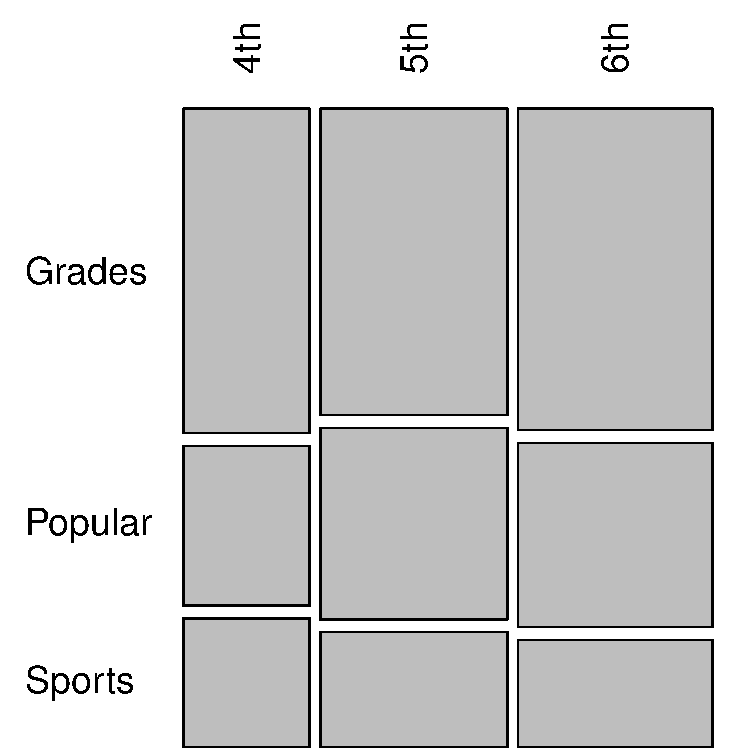
\includegraphics[width=0.8\textwidth]{6-4_chisq_indep/figures/popular/popular_mosaic}
\end{center}
}


\end{frame}

%%%%%%%%%%%%%%%%%%%%%%%%%%%%%%%%%%%

\begin{frame}
\frametitle{Chi-square test of independence}

\begin{itemize}
\item The hypotheses are:
\begin{itemize}
\item[$H_0$:] Grade and goals are independent. Goals do not vary by grade.
\item[$H_A$:] Grade and goals are dependent. Goals vary by grade.
\end{itemize}

\pause

\item The test statistic is calculated as
\[ \chi^2_{df} = \sum_{i = 1}^{k} \frac{(O - E)^2}{E} \quad \text{ where } \quad df = (R - 1) \times (C - 1), \]
where $k$ is the number of cells, $R$ is the number of rows, and $C$ is the number of columns.

\Note{We calculate $df$ differently for one-way and two-way tables.}

\pause

\item The p-value is the area under the $\chi^2_{df}$ curve, above the calculated test statistic.

\end{itemize}


\end{frame}

%%%%%%%%%%%%%%%%%%%%%%%%%%%%%%%%%%%

\subsection{Expected counts in two-way tables}

%%%%%%%%%%%%%%%%%%%%%%%%%%%%%%%%%%%

\begin{frame}
\frametitle{Expected counts in two-way tables}

\formula{Expected counts in two-way tables}
{
\[ \text{Expected Count} = \frac{(\text{row total}) \times (\text{column total})}{\text{table total}} \]
}

\pause

{\small
\begin{center}
\begin{tabular}{rrrr|r}
  \hline
 & Grades & Popular & Sports	& Total \\ 
  \hline
$4^{th}$ &  \orange{63} &  \green{31} &  25 	&119 \\ 
$5^{th}$ &  88 &  55 &  33	& 176 \\ 
$6^{th}$&  96 &  55 &  32	& 183 \\ 
   \hline
Total	& 247	& 141	& 90	& 478 \\
\end{tabular}
\end{center}
}

\pause

\[ \orange{$E_{row~1, col~1} = \frac{119 \times 247}{478} = 61$} \qquad \pause
 \green{$E_{row~1, col~2} = \frac{119 \times 141}{478} = 35$} \]

\end{frame}

%%%%%%%%%%%%%%%%%%%%%%%%%%%%%%%%%%%

\begin{frame}
\frametitle{Expected counts in two-way tables}

\pq{What is the expected count for the highlighted cell?}

{\small
\begin{center}
\begin{tabular}{rrrr|r}
  \hline
 & Grades & Popular & Sports	& Total \\ 
  \hline
$4^{th}$ &  63 &  31 &  25 	&119 \\ 
$5^{th}$ &  88 &  \orange{55} &  33	& 176 \\ 
$6^{th}$ &  96 &  55 &  32	& 183 \\ 
   \hline
Total	& 247	& 141	& 90	& 478 \\
\end{tabular}
\end{center}
}

\twocol{0.2}{0.8}
{
\begin{enumerate}[(a)]
\solnMult{$\frac{176 \times 141}{478}$}
\item $\frac{119 \times 141}{478}$
\item $\frac{176 \times 247}{478}$
\item $\frac{176 \times 478}{478}$
\end{enumerate}
}
{
\soln{\only<2>{
\orange{$\rightarrow$ 52\\
{\small more than expected \# of 5th graders \\
have a goal of being popular}}
\vspace{0.75cm}
}
}
}

\end{frame}

%%%%%%%%%%%%%%%%%%%%%%%%%%%%%%%%%%%

\begin{frame}
\frametitle{Calculating the test statistic in two-way tables}

Expected counts are shown in \ex{blue} next to the observed counts.
\begin{center}
\begin{tabular}{rrrr|r}
  \hline
 & Grades & Popular & Sports	& Total \\ 
  \hline
$4^{th}$ 	&  63 \ex{61} &  31 \ex{35} &  25 \ex{23}	&119 \\ 
$5^{th}$ 	&  88 \ex{91} &  55 \ex{52} &  33 \ex{33}	& 176 \\ 
$6^{th}$	&  96 \ex{95} &  55 \ex{54} &  32 \ex{34}	& 183 \\ 
   \hline
Total	& 247	& 141	& 90	& 478 \\
\end{tabular}
\end{center}

\vspace{0.5cm}

\pause

\begin{eqnarray*} 
\chi^2 &=& \sum \frac{(63 - 61)^2}{61} + \frac{(31 - 35)^2}{35} + \cdots + \frac{(32 - 34)^2}{34} = 1.3121 \\
\pause
df &=& (R - 1) \times (C - 1) = (3 - 1) \times (3 - 1) = 2 \times 2 = 4 
\end{eqnarray*}

\end{frame}

%%%%%%%%%%%%%%%%%%%%%%%%%%%%%%%%%%%

\subsection{Results}

%%%%%%%%%%%%%%%%%%%%%%%%%%%%%%%%%%%

\begin{frame}
\frametitle{Calculating the p-value}

\pq{Which of the following is the correct p-value for this hypothesis test?
\[ \chi^2 = 1.3121 \qquad df = 4 \]
}

\twocol{0.6}{0.4}{
\begin{center}
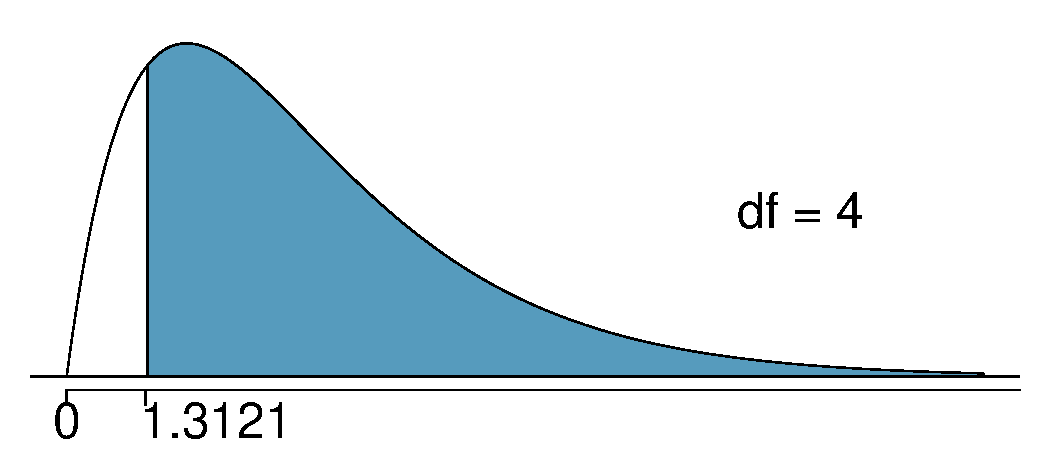
\includegraphics[width=0.67\textwidth]{6-4_chisq_indep/figures/popular/popular}
\end{center}
}
{
{\small
\begin{enumerate}[(a)]
\setlength{\itemsep}{0in}
\solnMult{ more than 0.3}
\item between 0.3 and 0.2
\item between 0.2 and 0.1
\item between 0.1 and 0.05
\item less than 0.001
\end{enumerate}
}
}

\begin{center}
{\scriptsize
\begin{tabular}{r | rrrr | rrrr |}
  \hline
Upper tail & 0.3 & 0.2 & 0.1 & 0.05 & 0.02 & 0.01 & 0.005 & 0.001 \\ 
  \hline
df \hfill 1 &  1.07 &  1.64 &  2.71 &  3.84 &  5.41 &  6.63 &  7.88 &  10.83 \\ 
  2 &  2.41 &  3.22 &  4.61 &  5.99 &  7.82 &  9.21 &  10.60 &  13.82 \\ 
  3 &  3.66 &  4.64 &  6.25 &  7.81 &  9.84 &  11.34 &  12.84 &  16.27 \\ 
  4 &  4.88 &  5.99 &  7.78 &  9.49 &  11.67 &  13.28 &  14.86 &  18.47 \\ 
  5 &  6.06 &  7.29 &  9.24 &  11.07 &  13.39 &  15.09 &  16.75 &  20.52 \\ 
\end{tabular}
}
\end{center}

\end{frame}

%%%%%%%%%%%%%%%%%%%%%%%%%%%%%%%%%%%

\begin{frame}
\frametitle{Conclusion}

\dq{Do these data provide evidence to suggest that goals vary by grade?}

\begin{itemize}

\item[$H_0$:] Grade and goals are independent. Goals do not vary by grade.

\item[$H_A$:] Grade and goals are dependent. Goals vary by grade. \\

\end{itemize}

$\:$ \\

\soln{\only<2>{Since p-value is high, we fail to reject $H_0$. The data do not provide convincing evidence that grade and goals are dependent. It doesn't appear that goals vary by grade.
}
}

\end{frame}

%%%%%%%%%%%%%%%%%%%%%%%%%%%%%%%%%%%%

\section{Small sample inference for a proportion}

%%%%%%%%%%%%%%%%%%%%%%%%%%%%%%%%%%%%

\subsection{Paul the octopus}

%%%%%%%%%%%%%%%%%%%%%%%%%%%%%%%%%%%%

\begin{frame}
\frametitle{Famous predictors}

\twocol{0.5}{0.5}{
Before this guy...
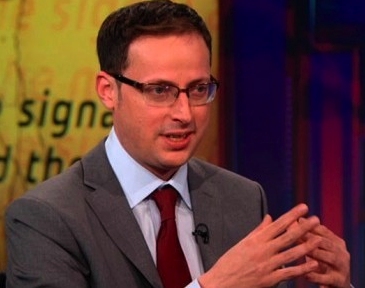
\includegraphics[width=\textwidth]{6-5_small_single_prop/figures/paul/nate}
}
{
\pause
There was this guy...
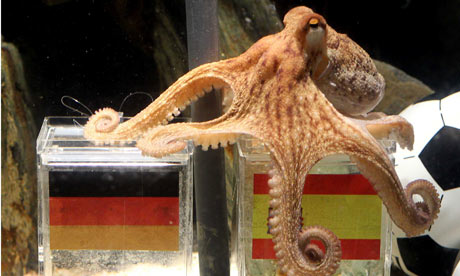
\includegraphics[width=\textwidth]{6-5_small_single_prop/figures/paul/paul}
}

\end{frame}

%%%%%%%%%%%%%%%%%%%%%%%%%%%%%%%%%%

\begin{frame}
\frametitle{Paul the Octopus - psychic?}

\begin{itemize}

\item Paul the Octopus predicted 8 World Cup games, and predicted them all correctly  

\pause

\item Does this provide convincing evidence that Paul actually has psychic powers?

\pause

\item How unusual would this be if he was just randomly guessing (with a 50\% chance of 
guessing correctly)?

\pause

\item Hypotheses:
\begin{itemize}
\item[$H_0:$] $p = 0.5$
\item[$H_A:$] $p > 0.5$
\end{itemize}

\end{itemize}

\end{frame}

%%%%%%%%%%%%%%%%%%%%%%%%%%%%%%%%%%

\begin{frame}
\frametitle{Conditions}

\begin{enumerate}

\item \hl{Independence:} We can assume that each guess is independent of another.

\pause

\item \hl{Sample size:} The number of expected successes is \orange{smaller than 10}.
\[ 8 \times 0.5 = 4 \]

\end{enumerate}

\pause

\vspace{1cm}

\dq{So what do we do?}

\pause

Since the sample size isn't large enough to use CLT based methods, we use a simulation method instead.

\end{frame}

%%%%%%%%%%%%%%%%%%%%%%%%%%%%%%%%%%

\begin{frame}
\frametitle{}

\pq{Which of the following methods is best way to calculate the p-value of the hypothesis test evaluating if Paul the Octopus' predictions are unusually higher than random guessing?}

\begin{enumerate}[(a)]
\item Flip a coin 8 times, record the proportion of times where all 8 tosses were heads. Repeat this many times, and calculate the proportion of simulations where all 8 tosses were heads.
\item Roll a die 8 times, record the proportion of times where all 8 rolls were 6s. Repeat this many times, and calculate the proportion of simulations where all 8 rolls were 6s.
\item Flip a coin 10,000 times, record the proportion of heads. Repeat this many times, and calculate the proportion of simulations where more than 50\% of tosses are heads.
\item Flip a coin 10,000 times, calculate the proportion of heads.
\end{enumerate}

\end{frame}

%%%%%%%%%%%%%%%%%%%%%%%%%%%%%%%%%%%

\begin{frame}
\frametitle{Simulate}

\pq{Flip a coin 8 times. Did you get all heads?}

\begin{enumerate}[(a)]
\item Yes
\item No
\end{enumerate}

\end{frame}

%%%%%%%%%%%%%%%%%%%%%%%%%%%%%%%%%%

\begin{frame}[fragile]
\frametitle{}

{\tiny
\begin{Verbatim}[frame=single, formatcom=\color{blue}]
source("http://www.openintro.org/stat/slides/inference.R")
paul = factor(c(rep("yes", 8), rep("no", 0)), levels = c("yes","no"))
inference(paul, est = "proportion", type = "ht", method = "simulation",
          success = "yes", null = 0.5, alternative = "greater", seed = 290)
\end{Verbatim}
}

\pause

{\tiny
\begin{Verbatim}[frame=single, formatcom=\color{gray}]
Single proportion -- success: yes 
Summary statistics: p_hat = 1 ;  n = 8 
H0: p = 0.5 
HA: p > 0.5 
p-value =  0.0037
\end{Verbatim}
}

\centering
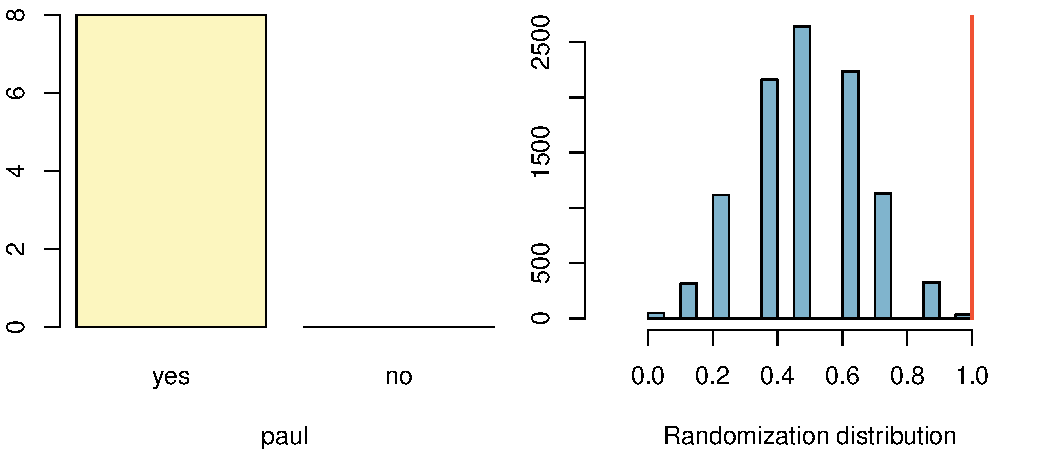
\includegraphics[width=0.8\textwidth,height=0.4\textheight]{6-5_small_single_prop/figures/paul/paul_HT}

\end{frame}

%%%%%%%%%%%%%%%%%%%%%%%%%%%%%%%%%%%

\begin{frame}
\frametitle{Conclusions}

\pq{Which of the following is \underline{false}?}

\begin{enumerate}[(a)]

\item If in fact Paul was randomly guessing, the probability that he would get the result of all 8 games correct is 0.0037.

\item Reject $H_0$, the data provide convincing evidence that Paul did better than randomly guessing.

\item We may have made a Type I error.

\solnMult{The probability that Paul is psychic is 0.0037.}

\end{enumerate}

\end{frame}

%%%%%%%%%%%%%%%%%%%%%%%%%%%%%%%%%%%%

\subsection{Back of the hand}

%%%%%%%%%%%%%%%%%%%%%%%%%%%%%%%%%%%

\begin{frame}
\frametitle{Back of the hand}

\dq{There is a saying ``know something like the back of your hand". Describe an experiment to test if people really do know the backs of their hands.}

\pause

\begin{center}
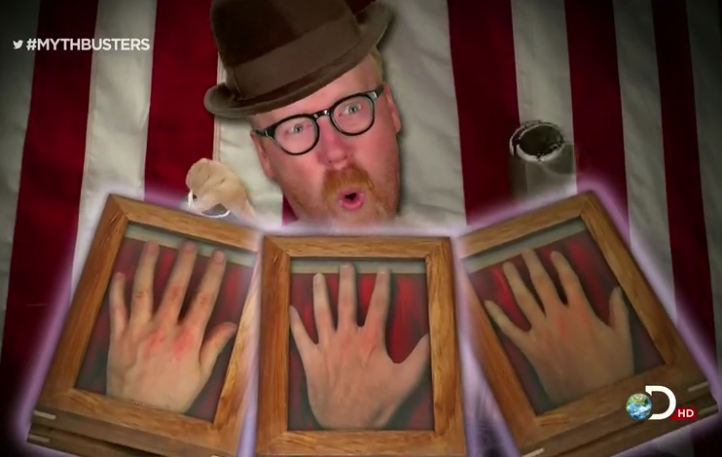
\includegraphics[width=0.6\textwidth]{6-5_small_single_prop/figures/hand/mythbusters}
\end{center}

In the MythBusters episode, 11 out of 12 people guesses the backs of their hands correctly.

\end{frame}

%%%%%%%%%%%%%%%%%%%%%%%%%%%%%%%%%%%%

\begin{frame}
\frametitle{Hypotheses}

\dq{What are the hypotheses for evaluating if people are capable of recognizing the back of their hand at a rate that is better than random guessing. Remember, in the MythBusters experiment, there were 10 pictures to choose from, and only 1 was correct.}

\begin{itemize}
\item[$H_0:$] $p = 0.10$ (random guessing)
\item[$H_A:$] $p > 0.10$ (better than random guessing)
\end{itemize}

\end{frame}

%%%%%%%%%%%%%%%%%%%%%%%%%%%%%%%%%%%

\begin{frame}
\frametitle{Conditions}

\begin{enumerate}

\item \hl{Independence:} We can assume that each person guessing is independent of another.

\item \hl{Sample size:} The number of expected successes is \orange{smaller than 10}.
\[ 12 \times 0.1 = 1.2 \]

\end{enumerate}

\dq{So what do we do?}

Since the sample size isn't large enough to use CLT based methods, we use a simulation method instead.

\end{frame}

%%%%%%%%%%%%%%%%%%%%%%%%%%%%%%%%%%%

\subsection{Randomization HT for a proportion}

%%%%%%%%%%%%%%%%%%%%%%%%%%%%%%%%%%%%

\begin{frame}
\frametitle{Simulation scheme}

\dq{Describe how you test if results of this experiment to determine if people are capable of recognizing the back of their hand at a rate that is better than random guessing.}
\vspace{-0.5cm}
\[ H_0: p = 0.10 \qquad H_A: p > 0.10 \qquad \hat{p} = 11 / 12 = 0.9167 \]

\begin{enumerate}

\item Use a 10-sided fair die to represent the sampling space, and call 1 a success (guessing correctly), and all other outcomes failures (guessing incorrectly).

\item Roll the die 12 times (representing 12 people in the experiment), count the number of 1s, and calculate the proportion of correct guesses in one simulation of 12 rolls.

\item Repeat step (2) many times, each time recording the proportion of successes in a series of 12 rolls of the die.

\item Create a dot plot of the simulated proportions from step (3) and count the number of simulations where the proportion was at least as high as 0.9167 (the observed proportion).

\end{enumerate}

\end{frame}

%%%%%%%%%%%%%%%%%%%%%%%%%%%%%%%%%%%

\begin{frame}
\frametitle{Simulation results}

\begin{itemize}

\item In the next slide you can see the results of a hypothesis test (using only 100 simulations to keep things simple).

\item Each dot represents a simulation proportion of success. There were 25-30 simulations where the success rate ($\hat{p}$) was 10\%, 40-45 simulations where the success rate was slightly less than 10\%, about 20 simulations where the success rate was slightly less than 20\% and 1 simulation where the success rate was more than 30\%.

\item There are no simulations where the success rate is as high as the observed success rate of 91.67\%.

\item Therefore we conclude that the observed result is near impossible to have happened by chance (p-value = 0).

\item And hence that these data suggest that people are capable of recognizing the back of their hand at a rate that is better than random guessing. 

\end{itemize}

\end{frame}

%%%%%%%%%%%%%%%%%%%%%%%%%%%%%%%%%%%%

\begin{frame}[fragile]
\frametitle{}

{\tiny
\begin{Verbatim}[frame=single, formatcom=\color{blue}]
back = as.factor(c(rep("correct", 11), rep("wrong", 1))) 
inference(back, est = "proportion", type = "ht", method = "simulation",
	success = "correct", null = 0.1, alternative = "greater", seed = 654, nsim = 100)
\end{Verbatim}
}

\pause

{\tiny
\begin{Verbatim}[frame=single, formatcom=\color{gray}]
Single proportion -- success: correct 
Summary statistics: p_hat = 0.9167 ;  n = 12 
H0: p = 0.1 
HA: p > 0.1 
p-value =  0 
\end{Verbatim}
}

\centering
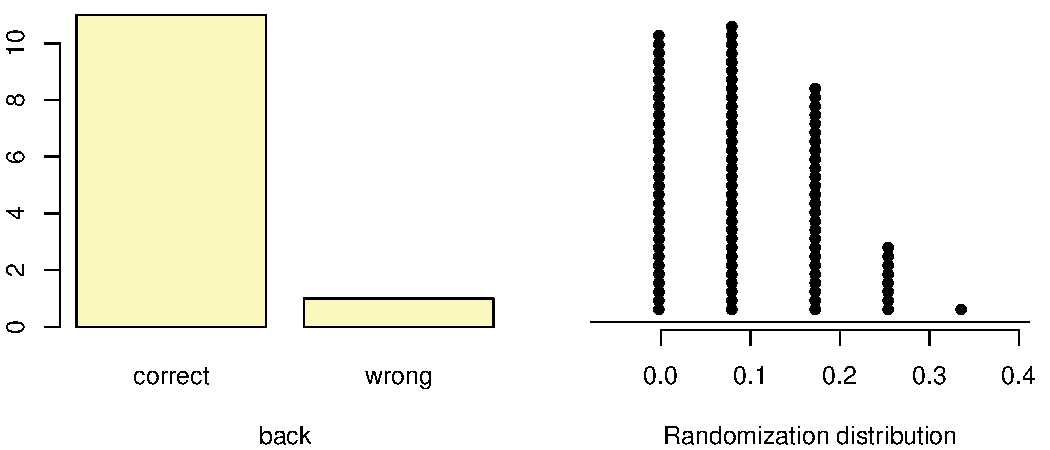
\includegraphics[width=0.8\textwidth,height=0.4\textheight]{6-5_small_single_prop/figures/hand/back_HT}

\end{frame}

%%%%%%%%%%%%%%%%%%%%%%%%%%%%%%%%%%%
%%%%%%%%%%%%%%%%%%%%%%%%%%%%%%%%%%%%

\section{Small sample inference for difference between two proportions}

%%%%%%%%%%%%%%%%%%%%%%%%%%%%%%%%%%%%

\begin{frame}
\frametitle{Comparing back of the hand to palm of the hand}

MythBusters also asked these people to guess the palms of their hands. This time 7 out of the 12 people guesses correctly. The data are summarized below.

\begin{center}
\begin{tabular}{ l | c | c | c }
          & Palm		& Back		& Total \\
\hline
Correct		& 11			& 7				& 18 \\
Wrong		  & 1				& 5				& 6 \\
\hline
Total			& 12			& 12			& 24 \\
\end{tabular}
\end{center}

\end{frame}

%%%%%%%%%%%%%%%%%%%%%%%%%%%%%%%%%%%%

\begin{frame}
\frametitle{Proportion of correct guesses}

{\small
\begin{center}
\begin{tabular}{ l | c | c | c }
          & Palm  	& Back		& Total \\
\hline
Correct		& 11			& 7				& 18 \\
Wrong		  & 1				& 5				& 6 \\
\hline
Total			& 12			& 12			& 24 \\
\end{tabular}
\end{center}

}

\begin{itemize}

\item Proportion of correct in the back group: $\frac{11}{12} = 0.916$

\item Proportion of correct in the palm group: $\frac{7}{12} = 0.583$

\item Difference: 33.3\% more correct in the back of the hand group.

\end{itemize}

\dq{Based on the proportions we calculated, do you think the chance of guessing the back of the hand correctly is different than palm of the hand?}

\end{frame}

%%%%%%%%%%%%%%%%%%%%%%%%%%%%%%%%%%%%

\begin{frame}
\frametitle{Hypotheses}

\dq{What are the hypotheses for comparing if the proportion of people who can guess the backs of their hands correctly is different than the proportion of people who can guess the palm of their hands correctly?}

\begin{itemize}
\item[$H_0$:] $p_{back} = p_{palm}$
\item[$H_0$:] $p_{back} \ne p_{palm}$
\end{itemize}

\end{frame}

%%%%%%%%%%%%%%%%%%%%%%%%%%%%%%%%%%%%

\begin{frame}
\frametitle{Conditions?}

\begin{itemize}

\item Independence - within groups, between groups?
\begin{itemize}
\item Within each group we can assume that the guess of one subject is independent of another.
\item Between groups independence is not satisfied - we have the same people guessing. However we'll assume they're independent guesses to continue with the analysis.
\end{itemize}

\item Sample size?
\begin{itemize}
\item $\hat{p}_{pool} = \frac{11 + 7}{12 + 12} = \frac{18}{24} = 0.75$
\item Expected successes in back group: $12 \times 0.75 = 9$, failures = 3
\item Expected successes in palm group: $12 \times 0.75 = 9$, failures = 3
\item Since S/F condition fails, we need to use simulation to compare the proportions.
\end{itemize}

\end{itemize}

\end{frame}

%%%%%%%%%%%%%%%%%%%%%%%%%%%%%%%%%%%%

\subsection{Randomization HT for comparing two proportions}

%%%%%%%%%%%%%%%%%%%%%%%%%%%%%%%%%%%%

\begin{frame}
\frametitle{Simulation scheme}

\begin{enumerate}

\item Use 24 index cards, where each card represents a subject.

\item Mark 18 of the cards as ``correct" and the remaining 6 as ``wrong".

\item Shuffle the cards and split into two groups of size 12, for back and palm.

\item Calculate the difference between the proportions of ``correct" in the back and palm decks, and record this number.

\item Repeat steps (3) and (4) many times to build a randomization distribution of differences in simulated proportions.

\end{enumerate}

\end{frame}

%%%%%%%%%%%%%%%%%%%%%%%%%%%%%%%%%%%%

\begin{frame}
\frametitle{Interpreting the simulation results}

When simulating the experiment under the assumption of independence, i.e. leaving things up to chance. \\

\vspace{0.5cm}

If results from the simulations based on the \hl{null model} look like the data, then we can determine that the difference between the proportions correct guesses in the two groups was simply \hl{due to chance}. \\

\vspace{0.5cm}

If the results from the simulations based on the null model do not look like the data, then we can determine that the difference between the proportions correct guesses in the two groups was not due to chance, but \hl{because people actually know the backs of their hands better}.

\end{frame}

%%%%%%%%%%%%%%%%%%%%%%%%%%%%%%%%%%%%

\begin{frame}
\frametitle{Simulation results}

\begin{itemize}

\item In the next slide you can see the result of a hypothesis test (using only 100 simulations to keep the results simple).

\item Each dot represents a difference in simulated proportion of successes. We can see that the distribution is centered at 0 (the null value).

\item We can also see that 9 out of the 100 simulations yielded simulated differences at least as large as the observed difference (p-value = 0.09).

\end{itemize}

\end{frame}

%%%%%%%%%%%%%%%%%%%%%%%%%%%%%%%%%%%%

\begin{frame}[fragile]
\frametitle{}

{\tiny
\begin{Verbatim}[frame=single, formatcom=\color{blue}]
hand = as.factor(c(rep("correct", 7), rep("wrong", 5), c(rep("correct", 11), rep("wrong", 1))))
gr = c(rep("palm",12),rep("back",12))
inference(hand, gr, est = "proportion", type = "ht", null = 0, alternative = "twosided",
	order = c("back","palm"), success = "correct", method = "simulation", seed = 879,
	nsim = 100)
\end{Verbatim}
}

\pause

{\tiny
\begin{Verbatim}[frame=single, formatcom=\color{gray}]
Response variable: categorical, Explanatory variable: categorical
Difference between two proportions -- success: correct
Summary statistics:
         x
y         back palm Sum
  correct   11    7  18
  wrong      1    5   6
  Sum       12   12  24
Observed difference between proportions (back-palm) = 0.3333
H0: p_back - p_palm = 0 
HA: p_back - p_palm != 0 
p-value =  0.18 
\end{Verbatim}
}

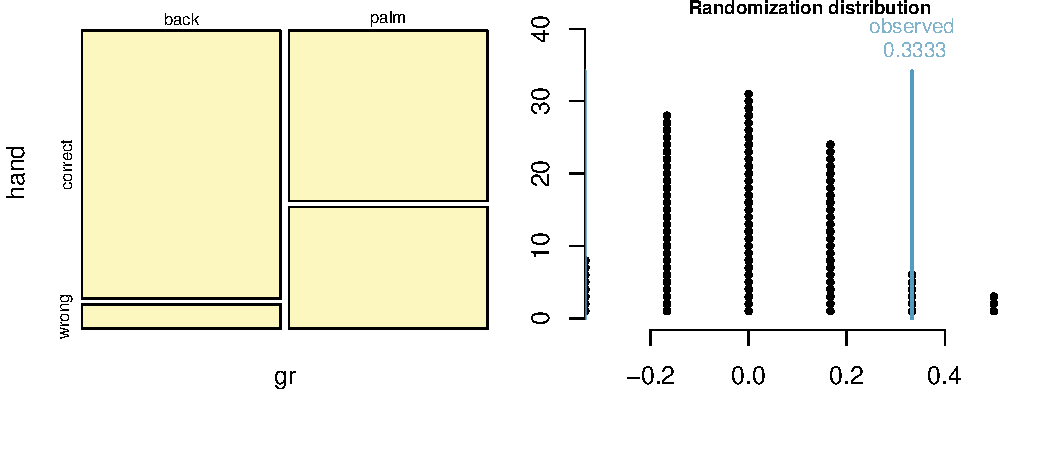
\includegraphics[width=0.8\textwidth,height=0.3\textheight]{6-6_small_two_props/figures/hand/palm_back_HT}

\end{frame}

%%%%%%%%%%%%%%%%%%%%%%%%%%%%%%%%%%%

\begin{frame}
\frametitle{Conclusion}

\pq{Do the simulation results suggest that people know the backs of their hands significantly better? \\
(Remember: There were 33.3\% more correct in the back group in the observed data.)}

\begin{enumerate}[(a)]
\item Yes
\solnMult{No}
\end{enumerate}

p-value = 0.09 $>$ 0.05, fail to reject $H_0$. The data do not provide convincing evidence that people know the backs of their hands better than the palms of their hands.

\end{frame}

%%%%%%%%%%%%%%%%%%%%%%%%%%%%%%%%%%%%%


%%%%%%%%%%%%%%%%%%%%%%%%%%%%%%%%%%%%
% End document
%%%%%%%%%%%%%%%%%%%%%%%%%%%%%%%%%%%%

\end{document}